% Options for packages loaded elsewhere
% Options for packages loaded elsewhere
\PassOptionsToPackage{unicode}{hyperref}
\PassOptionsToPackage{hyphens}{url}
\PassOptionsToPackage{dvipsnames,svgnames,x11names}{xcolor}
%
\documentclass[
  11pt,
]{article}
\usepackage{xcolor}
\usepackage[margin=1in]{geometry}
\usepackage{amsmath,amssymb}
\setcounter{secnumdepth}{5}
\usepackage{iftex}
\ifPDFTeX
  \usepackage[T1]{fontenc}
  \usepackage[utf8]{inputenc}
  \usepackage{textcomp} % provide euro and other symbols
\else % if luatex or xetex
  \usepackage{unicode-math} % this also loads fontspec
  \defaultfontfeatures{Scale=MatchLowercase}
  \defaultfontfeatures[\rmfamily]{Ligatures=TeX,Scale=1}
\fi
\usepackage{lmodern}
\ifPDFTeX\else
  % xetex/luatex font selection
\fi
% Use upquote if available, for straight quotes in verbatim environments
\IfFileExists{upquote.sty}{\usepackage{upquote}}{}
\IfFileExists{microtype.sty}{% use microtype if available
  \usepackage[]{microtype}
  \UseMicrotypeSet[protrusion]{basicmath} % disable protrusion for tt fonts
}{}
\usepackage{setspace}
\makeatletter
\@ifundefined{KOMAClassName}{% if non-KOMA class
  \IfFileExists{parskip.sty}{%
    \usepackage{parskip}
  }{% else
    \setlength{\parindent}{0pt}
    \setlength{\parskip}{6pt plus 2pt minus 1pt}}
}{% if KOMA class
  \KOMAoptions{parskip=half}}
\makeatother
% Make \paragraph and \subparagraph free-standing
\makeatletter
\ifx\paragraph\undefined\else
  \let\oldparagraph\paragraph
  \renewcommand{\paragraph}{
    \@ifstar
      \xxxParagraphStar
      \xxxParagraphNoStar
  }
  \newcommand{\xxxParagraphStar}[1]{\oldparagraph*{#1}\mbox{}}
  \newcommand{\xxxParagraphNoStar}[1]{\oldparagraph{#1}\mbox{}}
\fi
\ifx\subparagraph\undefined\else
  \let\oldsubparagraph\subparagraph
  \renewcommand{\subparagraph}{
    \@ifstar
      \xxxSubParagraphStar
      \xxxSubParagraphNoStar
  }
  \newcommand{\xxxSubParagraphStar}[1]{\oldsubparagraph*{#1}\mbox{}}
  \newcommand{\xxxSubParagraphNoStar}[1]{\oldsubparagraph{#1}\mbox{}}
\fi
\makeatother


\usepackage{longtable,booktabs,array}
\usepackage{calc} % for calculating minipage widths
% Correct order of tables after \paragraph or \subparagraph
\usepackage{etoolbox}
\makeatletter
\patchcmd\longtable{\par}{\if@noskipsec\mbox{}\fi\par}{}{}
\makeatother
% Allow footnotes in longtable head/foot
\IfFileExists{footnotehyper.sty}{\usepackage{footnotehyper}}{\usepackage{footnote}}
\makesavenoteenv{longtable}
\usepackage{graphicx}
\makeatletter
\newsavebox\pandoc@box
\newcommand*\pandocbounded[1]{% scales image to fit in text height/width
  \sbox\pandoc@box{#1}%
  \Gscale@div\@tempa{\textheight}{\dimexpr\ht\pandoc@box+\dp\pandoc@box\relax}%
  \Gscale@div\@tempb{\linewidth}{\wd\pandoc@box}%
  \ifdim\@tempb\p@<\@tempa\p@\let\@tempa\@tempb\fi% select the smaller of both
  \ifdim\@tempa\p@<\p@\scalebox{\@tempa}{\usebox\pandoc@box}%
  \else\usebox{\pandoc@box}%
  \fi%
}
% Set default figure placement to htbp
\def\fps@figure{htbp}
\makeatother


% definitions for citeproc citations
\NewDocumentCommand\citeproctext{}{}
\NewDocumentCommand\citeproc{mm}{%
  \begingroup\def\citeproctext{#2}\cite{#1}\endgroup}
\makeatletter
 % allow citations to break across lines
 \let\@cite@ofmt\@firstofone
 % avoid brackets around text for \cite:
 \def\@biblabel#1{}
 \def\@cite#1#2{{#1\if@tempswa , #2\fi}}
\makeatother
\newlength{\cslhangindent}
\setlength{\cslhangindent}{1.5em}
\newlength{\csllabelwidth}
\setlength{\csllabelwidth}{3em}
\newenvironment{CSLReferences}[2] % #1 hanging-indent, #2 entry-spacing
 {\begin{list}{}{%
  \setlength{\itemindent}{0pt}
  \setlength{\leftmargin}{0pt}
  \setlength{\parsep}{0pt}
  % turn on hanging indent if param 1 is 1
  \ifodd #1
   \setlength{\leftmargin}{\cslhangindent}
   \setlength{\itemindent}{-1\cslhangindent}
  \fi
  % set entry spacing
  \setlength{\itemsep}{#2\baselineskip}}}
 {\end{list}}
\usepackage{calc}
\newcommand{\CSLBlock}[1]{\hfill\break\parbox[t]{\linewidth}{\strut\ignorespaces#1\strut}}
\newcommand{\CSLLeftMargin}[1]{\parbox[t]{\csllabelwidth}{\strut#1\strut}}
\newcommand{\CSLRightInline}[1]{\parbox[t]{\linewidth - \csllabelwidth}{\strut#1\strut}}
\newcommand{\CSLIndent}[1]{\hspace{\cslhangindent}#1}



\setlength{\emergencystretch}{3em} % prevent overfull lines

\providecommand{\tightlist}{%
  \setlength{\itemsep}{0pt}\setlength{\parskip}{0pt}}



 


\makeatletter
\@ifpackageloaded{caption}{}{\usepackage{caption}}
\AtBeginDocument{%
\ifdefined\contentsname
  \renewcommand*\contentsname{Table of contents}
\else
  \newcommand\contentsname{Table of contents}
\fi
\ifdefined\listfigurename
  \renewcommand*\listfigurename{List of Figures}
\else
  \newcommand\listfigurename{List of Figures}
\fi
\ifdefined\listtablename
  \renewcommand*\listtablename{List of Tables}
\else
  \newcommand\listtablename{List of Tables}
\fi
\ifdefined\figurename
  \renewcommand*\figurename{Figure}
\else
  \newcommand\figurename{Figure}
\fi
\ifdefined\tablename
  \renewcommand*\tablename{Table}
\else
  \newcommand\tablename{Table}
\fi
}
\@ifpackageloaded{float}{}{\usepackage{float}}
\floatstyle{ruled}
\@ifundefined{c@chapter}{\newfloat{codelisting}{h}{lop}}{\newfloat{codelisting}{h}{lop}[chapter]}
\floatname{codelisting}{Listing}
\newcommand*\listoflistings{\listof{codelisting}{List of Listings}}
\makeatother
\makeatletter
\makeatother
\makeatletter
\@ifpackageloaded{caption}{}{\usepackage{caption}}
\@ifpackageloaded{subcaption}{}{\usepackage{subcaption}}
\makeatother
\usepackage{bookmark}
\IfFileExists{xurl.sty}{\usepackage{xurl}}{} % add URL line breaks if available
\urlstyle{same}
\hypersetup{
  pdftitle={Walk-Forward Physics-Informed Neural Networks for Option Pricing with Learnable Volatility and Arbitrage Diagnostics},
  pdfauthor={Darli Seranaj},
  colorlinks=true,
  linkcolor={blue},
  filecolor={Maroon},
  citecolor={Blue},
  urlcolor={Blue},
  pdfcreator={LaTeX via pandoc}}


\title{Walk-Forward Physics-Informed Neural Networks for Option Pricing
with Learnable Volatility and Arbitrage Diagnostics}
\author{Darli Seranaj}
\date{2026-05-02}
\begin{document}
\maketitle
\begin{abstract}
We benchmark physics-informed neural networks (PINNs) for option pricing
on a single-name equity dataset (TSLA, 2020) under a strict walk-forward
protocol. Stage 1 establishes a 13-configuration architecture ablation
under a single-phase val-best reporting scheme. Stage 2 replaces the
constant-volatility assumption inside the PDE with a learnable surface
\(\sigma_\theta(F,\tau)\) parametrized either multiplicatively (C-Vol)
or directly (A-Vol). Across all stages we treat butterfly and calendar
arbitrage violation rates as primary metrics on equal footing with RMSE.
Honest non-PINN baselines (Black--Scholes with per-fold ATM-\(\sigma\),
residual GAM, residual laGP) are evaluated under identical fold
definitions and information set. We outline an anchored-ensemble
uncertainty quantification scheme as a forward-looking extension.
\end{abstract}


\setstretch{1.15}
\pagebreak

\section{Introduction}\label{introduction}

The Black--Scholes formula (Black and Scholes 1973; Merton 1973) remains
the reference language of derivatives pricing despite decades of
empirical evidence that its constant-volatility assumption is wrong. The
two dominant responses (calibrating local or stochastic volatility
models (Dupire 1994; Heston 1993), or fitting flexible machine-learning
regressors to market quotes) solve different parts of the problem and
inherit different limitations. Calibration imposes structure but suffers
parameter instability across regimes. Pure ML methods deliver fit but
offer no guarantee that the resulting prices are even \emph{internally
consistent}: arbitrage violations such as butterfly or calendar
negatives are routinely tolerated because they are rarely measured.

Physics-informed neural networks (PINNs) (Raissi, Perdikaris, and
Karniadakis 2019) are appealing in this setting because they enforce the
pricing PDE as a soft constraint during training. In principle, this
combines the structural discipline of model-based pricing with the
flexibility of neural function approximation. In practice, the PINN
literature on options pricing has three recurrent gaps:

\begin{enumerate}
\def\labelenumi{\arabic{enumi}.}
\tightlist
\item
  experiments use synthetic data or single in-sample fits rather than
  walk-forward backtests;
\item
  the volatility entering the PDE is held \emph{constant}, identical to
  a single-\(\sigma\) Black--Scholes baseline, eliminating the very
  degree of freedom the network is meant to learn;
\item
  no-arbitrage properties of the trained surface are reported only when
  they happen to be clean.
\end{enumerate}

This paper closes those three gaps on a single-name equity option
dataset (TSLA, 2020). Our contributions are:

\begin{enumerate}
\def\labelenumi{\arabic{enumi}.}
\item
  Walk-forward PINN benchmark. Nine monthly folds across 2020, strict
  val-best snapshot reporting, and a 13-configuration architecture
  ablation (random weight factorization \(\mu\) \times loss-balancing
  strategy \times hybrid vs.~physics-only mode). Stage 1 establishes
  that with appropriate Modified-MLP + RWF + Fourier-feature
  architecture (Wang et al. 2023; Tancik et al. 2020) and a PDE-warmup
  schedule, the PINN matches a per-fold-\(\sigma\) Black--Scholes
  baseline on pooled RMSE while introducing a \emph{wing inversion} in
  stratified error: the only configuration in our ablation grid where
  out-of-the-money and in-the-money RMSE both improve relative to
  at-the-money.
\item
  Stage 2: learnable \(\sigma\) surface. We replace the
  constant-\(\sigma\) assumption inside the PDE with a learned surface
  \(\sigma_\theta(F,\tau)\) realised via two parametrizations: a
  multiplicative \emph{C-Vol} wrapper
  \(\sigma(F,\tau) = \sigma_0 \cdot \mathrm{softplus}(g_\theta(F,\tau))\)
  and a direct \emph{A-Vol} parametrization
  \(\sigma(F,\tau) = \sigma_\mathrm{init} + \mathrm{softplus}(g_\theta(F,\tau))\).
  Both are warm-started from the two endpoints of the Stage 1 ablation:
  B10 (best pricing accuracy, structural arb violations) and B12
  (cleanest no-arb surface, marginally worse pricing).
\item
  Arbitrage as a first-class metric. Every reported model is evaluated
  for butterfly and calendar arbitrage on a dense \((F,\tau)\) grid. We
  treat the violation rate as a primary metric on equal footing with
  RMSE, exposing the trade-off that pure-RMSE reporting conceals.
\item
  Honest non-PINN baselines. A residual GAM (Wood 2017) and a local
  approximate Gaussian process (Gramacy 2016) are evaluated under
  identical walk-forward folds and the strict feature set the PINN sees,
  removing regime-indicator contamination present in earlier
  formulations. The laGP fit additionally produces native 95\%
  predictive intervals that we retain as the comparison baseline for the
  uncertainty extension outlined in Section \ref{sec-discussion}.
\end{enumerate}

\begin{longtable}[]{@{}llllll@{}}
\caption{Headline results: pooled RMSE in dollars and arbitrage
violation rates across baseline classes. The wing-inversion case (wing
RMSE below ATM RMSE) appears only in the B10
configuration.}\label{tbl-headline}\tabularnewline
\toprule\noalign{}
Config & RMSE & ATM & Wing & Butt \% & Cal \% \\
\midrule\noalign{}
\endfirsthead
\toprule\noalign{}
Config & RMSE & ATM & Wing & Butt \% & Cal \% \\
\midrule\noalign{}
\endhead
\bottomrule\noalign{}
\endlastfoot
BS & 8.795 & --- & --- & --- & --- \\
GAM & 9.305 & 9.272 & 9.313 & --- & --- \\
LAGP & 11.305 & 11.113 & 11.350 & --- & --- \\
B0 & 9.032 & 8.864 & 9.072 & 3.680 & 0.260 \\
B1 & 8.698 & 8.560 & 8.730 & 6.560 & 0.570 \\
B10 & 8.487 & 8.828 & 8.402 & 32.010 & 18.960 \\
B12 & 8.746 & 8.480 & 8.809 & 21.200 & 1.670 \\
\end{longtable}

The remainder of the paper is organized as follows. Section
\ref{sec-background} reviews the necessary PDE and PINN background.
Section \ref{sec-methodology} details data preprocessing, walk-forward
methodology, and the three-stage architecture. Section \ref{sec-stage1}
presents Stage 1 ablation results. Section \ref{sec-stage2} the Stage 2
vol-surface results. Section \ref{sec-baselines} compares against
non-PINN baselines. Section \ref{sec-discussion} discusses limitations
and outlines the uncertainty-quantification extension; Section
\ref{sec-conclusion} concludes.

\pagebreak

\section{Background}\label{sec-background}

\subsection{The Black--Scholes pricing
PDE}\label{the-blackscholes-pricing-pde}

For a European call on a non-dividend-paying underlying \(S_t\) under
the risk-neutral measure with constant interest rate \(r\) and
volatility \(\sigma\), the option price \(V(S,t)\) satisfies

\begin{equation}\phantomsection\label{eq-bs-pde}{
\frac{\partial V}{\partial t}
+ \frac{1}{2}\sigma^2 S^2 \frac{\partial^2 V}{\partial S^2}
+ r S \frac{\partial V}{\partial S} - r V = 0,
}\end{equation}

with terminal condition \(V(S, T) = (S - K)^+\) and boundary conditions
\(V(0, t) = 0\), \(V(S, t) \to S - K e^{-r(T-t)}\) as \(S \to \infty\).

We work in non-dimensionalised coordinates throughout: moneyness
\(m = F/K\) where \(F = S e^{(r-q)(T-t)}\) is the forward price, time to
expiry \(\tau = T - t\), and price \(\hat v = V/K\).

\subsection{Physics-informed neural
networks}\label{physics-informed-neural-networks}

A PINN \(\hat v_\phi(m,\tau)\) is trained to minimise a composite loss

\begin{equation}\phantomsection\label{eq-loss}{
\mathcal{L}(\phi) = \lambda_\mathrm{pde}\mathcal{L}_\mathrm{pde}
+ \lambda_\mathrm{tc}\mathcal{L}_\mathrm{tc}
+ \lambda_\mathrm{bc}\mathcal{L}_\mathrm{bc}
+ \lambda_\mathrm{data}\mathcal{L}_\mathrm{data}
+ \lambda_\mathrm{reg}\mathcal{L}_\mathrm{reg},
}\end{equation}

where \(\mathcal{L}_\mathrm{pde}\) is the squared residual of
Equation~\ref{eq-bs-pde} at collocation points,
\(\mathcal{L}_\mathrm{tc}\) and \(\mathcal{L}_\mathrm{bc}\) enforce
terminal and boundary conditions, \(\mathcal{L}_\mathrm{data}\) is the
mean squared error against market mid-prices, and
\(\mathcal{L}_\mathrm{reg}\) regularises soft-plus arguments. The
adaptive weights \(\{\lambda_i\}\) are updated via the gradient-norm
scheme of Wang et al. (2023).

\subsection{No-arbitrage diagnostics}\label{no-arbitrage-diagnostics}

A theoretical option price surface \(V(K,\tau)\) must satisfy two
inequalities almost everywhere:

\begin{equation}\phantomsection\label{eq-butterfly}{
\frac{\partial^2 V}{\partial K^2} \ge 0
\quad\text{(butterfly, convexity in strike)},
}\end{equation}

\begin{equation}\phantomsection\label{eq-calendar}{
\frac{\partial V}{\partial \tau} \ge 0
\quad\text{(calendar, monotonicity in maturity)}.
}\end{equation}

We measure violation rates by Monte Carlo over a dense \((K,\tau)\)
grid; see Section \ref{sec-methodology} for the implementation.

\pagebreak

\section{Methodology}\label{sec-methodology}

The three stages compose incrementally: Stage 1 inherits Stage 0's PDE
residual + boundary conditions and adds Modified-MLP, Random Weight
Factorization, Fourier-feature inputs, gradient-norm balancing, the
market-data loss, walk-forward folds, and val-best snapshot reporting;
Stage 2 inherits all of that and adds a learned
\(\sigma_\theta(F,\tau)\) network jointly trained with a warm-started
pricing net (Figure \ref{fig-architecture}).

\begin{figure}[H]

\centering{

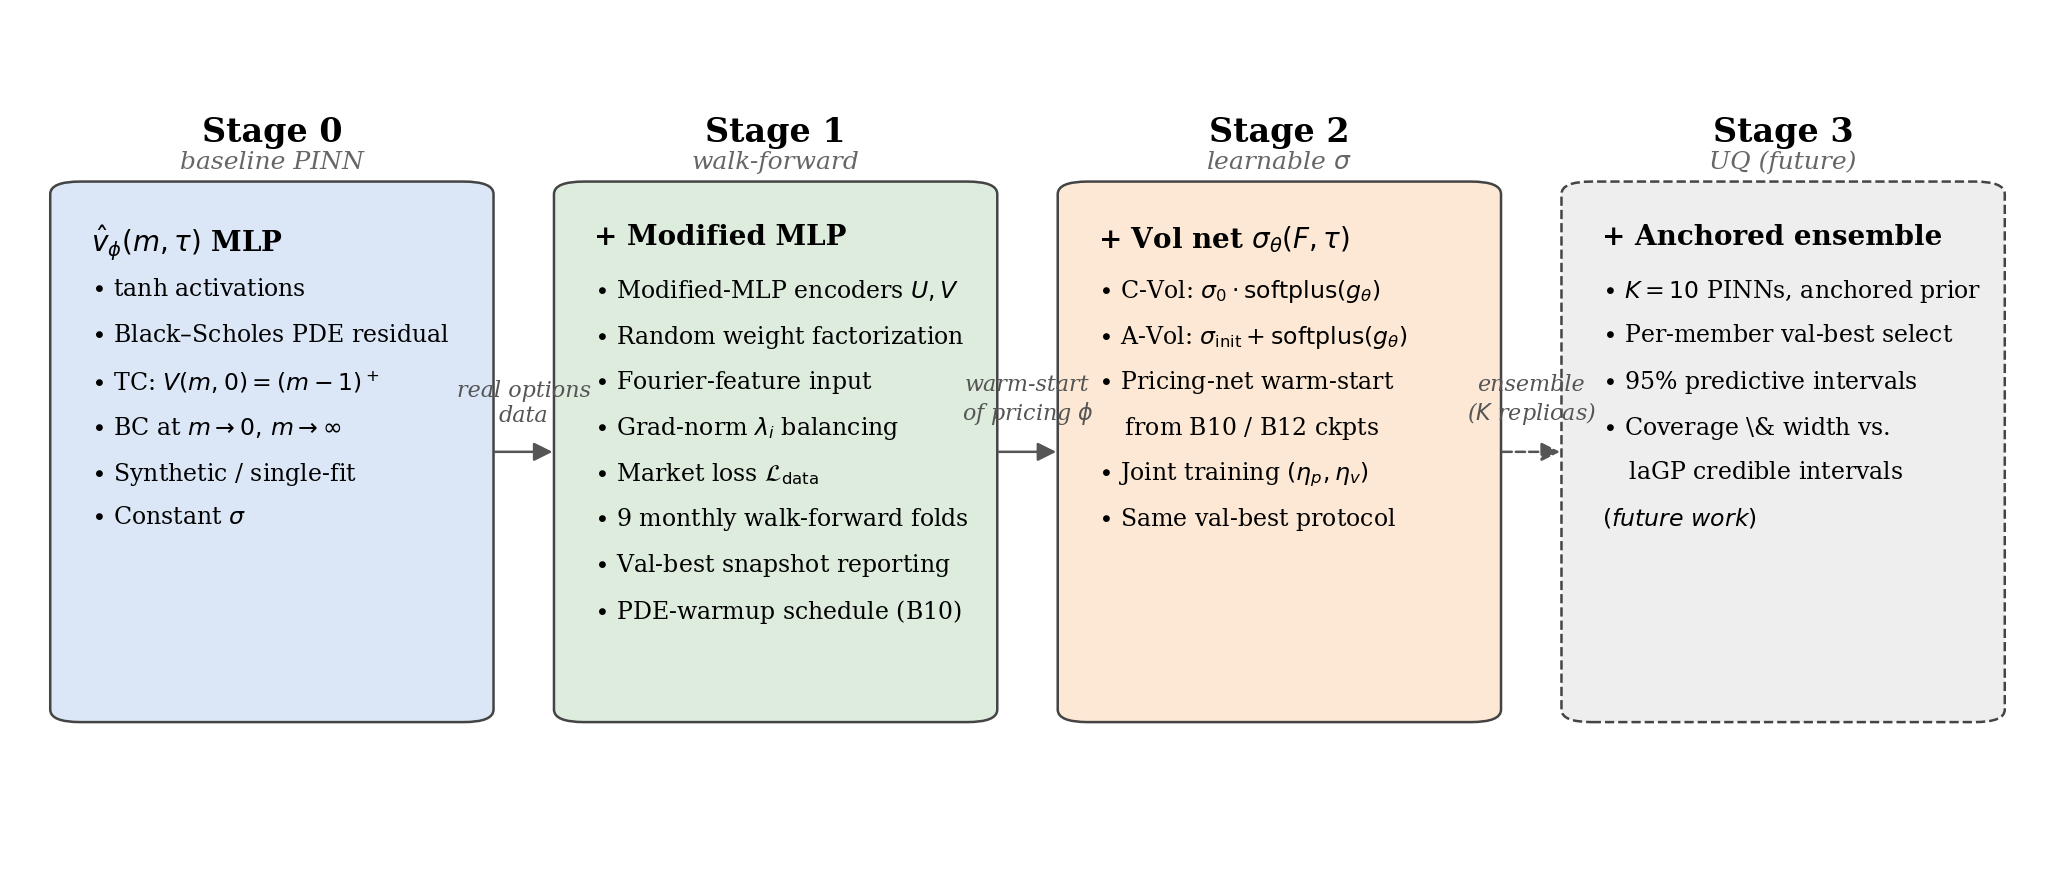
\includegraphics[width=1\linewidth,height=\textheight,keepaspectratio]{figures/fig-architecture.png}

}

\caption{\label{fig-architecture}Method evolution. Stage 0 baseline
PINN; Stage 1 walk-forward PINN with Modified-MLP/RWF/Fourier-feature
pricing net and grad-norm-balanced losses; Stage 2 jointly-trained
learnable volatility surface; Stage 3 (future) anchored ensemble for
uncertainty quantification.}

\end{figure}%

\subsection{Data and walk-forward
folds}\label{data-and-walk-forward-folds}

We use end-of-day TSLA option chain quotes from 2020, split-adjusted for
the August 2020 5:1 stock split. After standard cleaning (positive
mid-price, in-the-money intrinsic value bounds, removal of zero-volume
quotes), the cleaned panel contains 59,668 option-day observations
across 252 trading days.

Folds are monthly and walk-forward: for fold \(f\) (test month \(M_f\)),
training spans all data strictly before the start of \(M_{f-1}\), the
last calendar month of training is held out as the validation set
\(M_{f-1}\), and the test set is \(M_f\) (Figure \ref{fig-walkforward}).
This yields nine folds covering April through December 2020. Per-fold
constants are computed \emph{only} from training data:
\(\sigma_\mathrm{fixed}\) is the median of ATM implied volatilities and
\(r_\mathrm{fixed}\) the cross-sectional mean of risk-free rates.

\begin{figure}[H]

\centering{

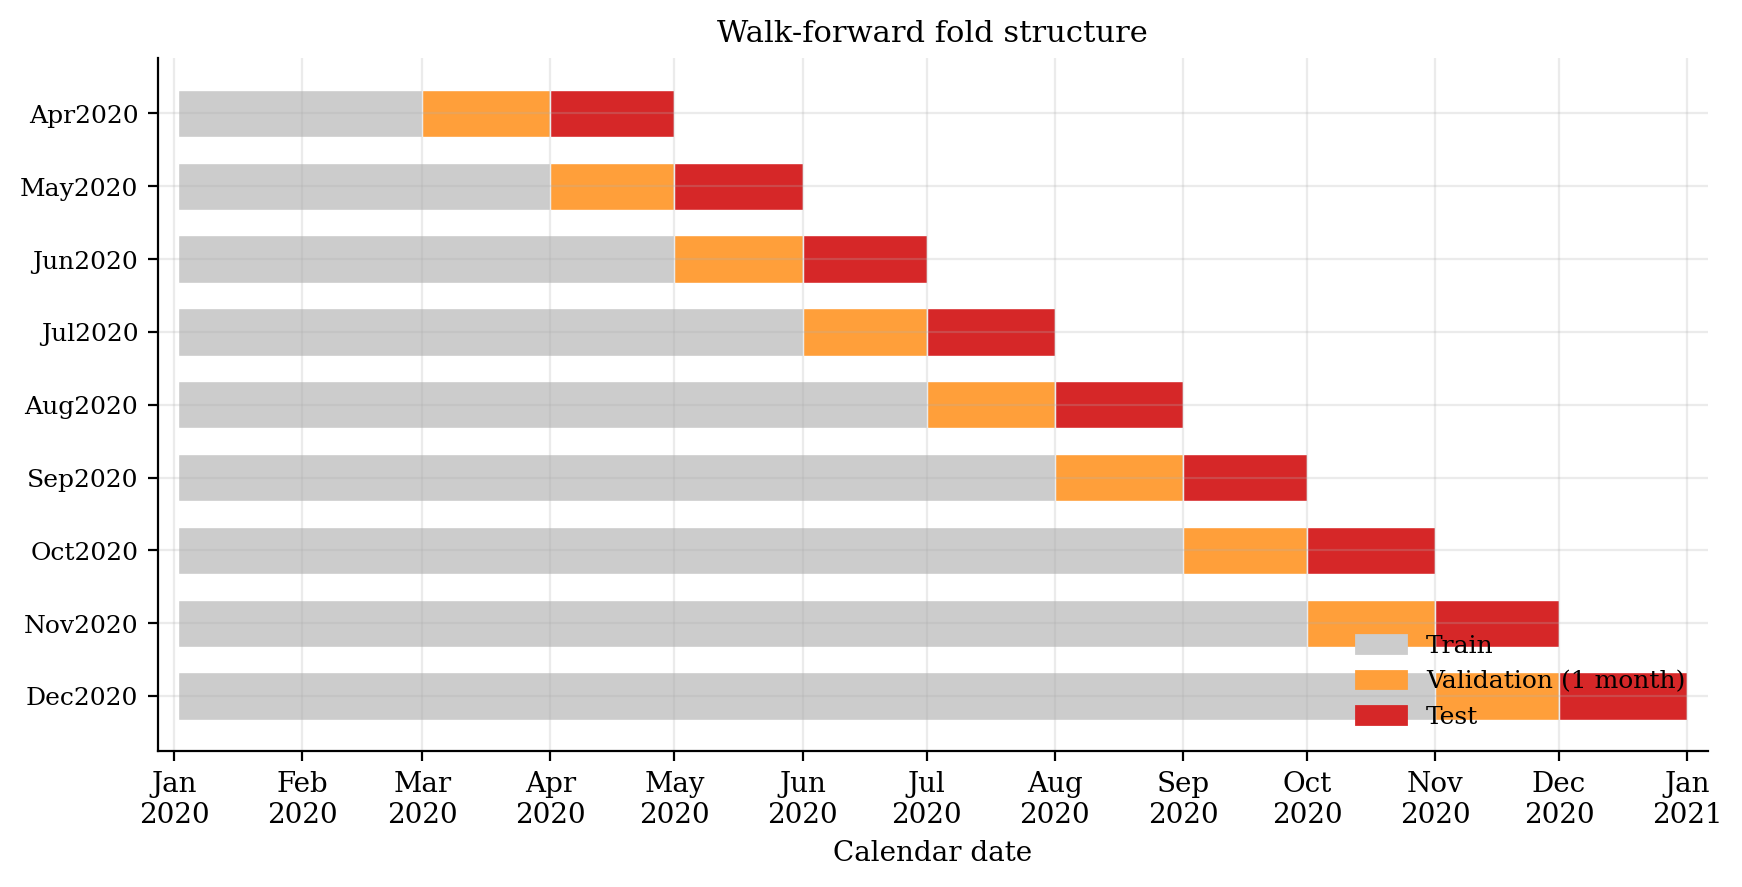
\includegraphics[width=0.9\linewidth,height=\textheight,keepaspectratio]{figures/fig-walkforward-timeline.png}

}

\caption{\label{fig-walkforward}Walk-forward fold structure. For each
fold \(f\), the model is trained on data strictly preceding the
validation window \(M_{f-1}\) (gray), with \(M_{f-1}\) used only to
drive val-best snapshot selection (orange), and reported on the held-out
test month \(M_f\) (red). The training window grows monotonically across
folds.}

\end{figure}%

\subsection{PINN architecture}\label{pinn-architecture}

The pricing network is a Modified-MLP (Wang et al. 2023), an
encoder-gated multi-layer perceptron whose two parallel encoder streams
give the network better gradient flow than a vanilla MLP of equivalent
depth, which matters because the PDE residual asks for stable
second-order derivatives. Inputs pass first through a Fourier feature
embedding (Tancik et al. 2020), which expands the low-dimensional input
\((m,\tau)\) into a higher-dimensional sinusoidal basis; this is what
allows the network to capture the high-frequency curvature of the
volatility smile without saturating its early layers on essentially-flat
low-frequency features. Every linear layer is reparametrised with Random
Weight Factorization (RWF) \(\mathbf{W} = \mathrm{diag}(s)\,
\hat{\mathbf{W}}\) with scale vector \(s \sim \mathcal{N}(\mu,
\sigma_\mathrm{init}^2)\); this rescales the per-neuron gradient norms
so that grad-norm balancing (Section \ref{sec-training}) does not have
to cancel pathological per-layer gradient magnitudes before it can
balance the \emph{loss-term} gradients we actually care about. All
activations are \(\tanh\) to permit second-order autograd for the PDE
residual.

We sweep a \(\mu \in \{0.0, 0.25, 0.5, 0.75, 1.0\}\) ablation in
combination with: hybrid vs.~physics-only loss, fixed vs.
gradient-norm-balanced data weight, and PDE-warmup vs.~immediate-data
training. The full grid is reported in Section \ref{sec-stage1}.

\subsection{Training protocol}\label{sec-training}

The composite loss in Equation \ref{eq-loss} mixes terms with very
different gradient magnitudes (the PDE residual is naturally
\(O(10^{-2})\), the market-data MSE is \(O(10^{0})\) in non-dimensional
units), so a fixed weighting collapses one term against another. We
adopt the gradient-norm scheme of Wang et al. (2023): every
\(T_g{=}100\) epochs the active loss weights are updated as

\begin{equation}\phantomsection\label{eq-grad-norm}{
\lambda_i \;\leftarrow\; (1-\alpha)\,\lambda_i
+ \alpha \cdot \frac{\max_j \lVert \nabla_\phi \mathcal{L}_j \rVert}
                     {\lVert \nabla_\phi \mathcal{L}_i \rVert + \varepsilon},
\qquad \alpha = 0.1,
}\end{equation}

with \(\nabla_\phi\) over all trainable pricing-net parameters. The
weights for the terminal- and boundary-condition terms
\((\lambda_\mathrm{tc},\lambda_\mathrm{bc})\) are floored at 10 to
prevent the scheme from sending them to zero on long runs.

\subsubsection{Two overfitting modes}\label{two-overfitting-modes}

PINN-pricing under the hybrid loss admits two distinct overfitting
dynamics that we have to control for separately:

\begin{itemize}
\item
  Generic supervised overfitting. \(\mathcal{L}_\mathrm{data}\)
  continues to admit arbitrarily small training error as the network
  increases capacity to fit idiosyncratic mid-quote noise. This is the
  textbook supervised failure mode and the val-best mechanism below is
  the standard defence against it.
\item
  Gradient-norm collapse (the PINN-specific failure). The gradient-norm
  scheme of Equation \ref{eq-grad-norm} amplifies whichever term has the
  largest gradient. Because \(\mathcal{L}_\mathrm{data}\) decreases more
  slowly than the PDE / TC / BC terms in late training, the scheme keeps
  lifting \(\lambda_\mathrm{data}\) to compensate. Once it drifts far
  enough, the \emph{PDE dominance ratio}
  \(\rho(t) = \lambda_\mathrm{pde}\mathcal{L}_\mathrm{pde}/
  (\lambda_\mathrm{tc}\mathcal{L}_\mathrm{tc} +
  \lambda_\mathrm{bc}\mathcal{L}_\mathrm{bc})\) falls below unity and
  the optimiser is pulled away from PDE-consistent solutions toward
  arbitrage-violating minima of the data loss. Section
  \ref{sec-stability} documents this regime empirically; the PDE-warmup
  schedule defined later in this section is the structural fix that
  prevents it from ever being reached.
\end{itemize}

\subsubsection{Val-best snapshot
reporting}\label{val-best-snapshot-reporting}

To guard against both modes simultaneously without conflating them, each
fold uses a single training run with val-best snapshot reporting:

\begin{enumerate}
\def\labelenumi{\arabic{enumi}.}
\tightlist
\item
  Initialise the model with seed \(S=42\).
\item
  Train for \(E_\mathrm{max}=15,000\) epochs on the train window only;
  evaluate val RMSE every \(T_v{=}250\) epochs.
\item
  Snapshot the full \((\phi, \theta)\) state whenever val RMSE improves
  on the running best.
\item
  After the loop, restore the val-best snapshot and evaluate the test
  month \emph{once}. Reported numbers are this single post-restore
  evaluation.
\end{enumerate}

The reported epoch \(E^\star\) is therefore the last point at which the
val curve was still improving, a deterministic readout of the fold's
effective training horizon. Test data are touched exactly once per fold;
the val window is held out from training and used \emph{only} to drive
snapshot selection. Saved checkpoints are the val-best states; Stage 2
warm-starts from the same val-best \(\phi\), so the val window is held
out from Stage 2's optimisation horizon as well.

\subsubsection{PDE-warmup schedule}\label{pde-warmup-schedule}

For configurations with \texttt{-\/-data\_loss\_warmup} \(= W > 0\)
(B10--B12 in our grid), the data term is \emph{deactivated} for the
first \(W\) epochs: the model is trained as a physics-only PINN (PDE +
TC + BC residuals), letting the gradient-norm scheme settle on a
balanced
\((\lambda_\mathrm{pde},\lambda_\mathrm{tc},\lambda_\mathrm{bc})\)
inside a region of parameter space where the no-arbitrage geometry is
established. At epoch \(W{+}1\) the data term is admitted with
\(\lambda_\mathrm{data}\!\leftarrow\!1\), and joint gradient-norm
balancing resumes. The warmup window \(W{=}5,000\) was selected
empirically as the point at which \(\rho(t) \to O(1)\) for the
physics-only run; longer warmups provide diminishing returns, shorter
warmups fail to establish the balance before
\(\mathcal{L}_\mathrm{data}\) is admitted. The ablation in Section
\ref{sec-stage1} shows that this single schedule choice, together with
the val-best snapshot, is responsible for the gap between the
hybrid-collapse configurations (B5--B7) and the Pareto-frontier
configurations (B10--B12).

\subsection{Stage 2: learnable
volatility}\label{stage-2-learnable-volatility}

A second network \(g_\theta(F,\tau)\) produces the volatility surface.
We compare two parametrizations:

\begin{equation}\phantomsection\label{eq-vol-params}{
\sigma_\mathrm{C}(F,\tau)
  = \sigma_0 \cdot \mathrm{softplus}\bigl(g_\theta(F,\tau)\bigr),
\qquad
\sigma_\mathrm{A}(F,\tau)
  = \sigma_\mathrm{init} + \mathrm{softplus}\bigl(g_\theta(F,\tau)\bigr),
}\end{equation}

where \(\sigma_0\) is the per-fold-\(\sigma_\mathrm{fixed}\) anchor
(C-Vol) and \(\sigma_\mathrm{init}\) is the same value used as an
additive offset (A-Vol). The pricing network is warm-started from a
Stage 1 fold checkpoint; the volatility network is trained from scratch
with its own learning rate \(\eta_\mathrm{vol} = 10^{-3}\), above the
pricing fine-tune rate \(\eta_\mathrm{price} = 10^{-4}\).

\subsection{Baselines}\label{sec-baselines-method}

Three non-PINN baselines run on identical fold definitions:

\begin{itemize}
\tightlist
\item
  A1: Black--Scholes (per-fold \(\sigma\)). Closed-form
  Equation~\ref{eq-bs-pde} with \(\sigma = \sigma_\mathrm{fixed}\) and
  \(r = r_\mathrm{fixed}\) both computed from training data only.
\item
  A2: Residual GAM. Target is \(y = \mathrm{mid} - V_\mathrm{BS}\), fit
  with \texttt{mgcv::gam} using
  \(y \sim \mathrm{te}(m,\tau,k=(8,5)) + \mathrm{ns}(\log v, \mathrm{df}=2)\),
  REML smoothing.
\item
  A3: Residual laGP. Same target as A2; local approximate GP with
  start=6, end=50 (Gramacy 2016), yielding native 95\% predictive
  intervals retained as the credible-interval baseline for the
  uncertainty extension in Section \ref{sec-uq-future}.
\end{itemize}

\pagebreak

\section{Stage 1: Walk-forward ablation}\label{sec-stage1}

\begin{longtable}[]{@{}
  >{\raggedright\arraybackslash}p{(\linewidth - 20\tabcolsep) * \real{0.1031}}
  >{\raggedright\arraybackslash}p{(\linewidth - 20\tabcolsep) * \real{0.0928}}
  >{\raggedright\arraybackslash}p{(\linewidth - 20\tabcolsep) * \real{0.0928}}
  >{\raggedright\arraybackslash}p{(\linewidth - 20\tabcolsep) * \real{0.1031}}
  >{\raggedright\arraybackslash}p{(\linewidth - 20\tabcolsep) * \real{0.0825}}
  >{\raggedright\arraybackslash}p{(\linewidth - 20\tabcolsep) * \real{0.0825}}
  >{\raggedright\arraybackslash}p{(\linewidth - 20\tabcolsep) * \real{0.0825}}
  >{\raggedright\arraybackslash}p{(\linewidth - 20\tabcolsep) * \real{0.0825}}
  >{\raggedright\arraybackslash}p{(\linewidth - 20\tabcolsep) * \real{0.0825}}
  >{\raggedright\arraybackslash}p{(\linewidth - 20\tabcolsep) * \real{0.1031}}
  >{\raggedright\arraybackslash}p{(\linewidth - 20\tabcolsep) * \real{0.0928}}@{}}
\caption{Full Stage 1 ablation (B0--B12) with the architectural
parameters that distinguish each cell (loss type, RWF \(\mu\), and
PDE-warmup window (epochs)) followed by pooled RMSE in dollars across
all 9 folds and the butterfly / calendar arbitrage violation rates. B0
and B1 use the standard MLP architecture (no RWF, hence no \(\mu\)
entry). B9 shares its three-parameter signature with B6 but additionally
pins \(\lambda_\mathrm{data}=1000\) instead of using gradient-norm
balancing. The wing-inversion case (wing RMSE below ATM RMSE) appears
only in B10 (modified-hybrid, \(\mu = 0.75\), warmup =
5000).}\label{tbl-stage1}\tabularnewline
\toprule\noalign{}
\begin{minipage}[b]{\linewidth}\raggedright
Config
\end{minipage} & \begin{minipage}[b]{\linewidth}\raggedright
Loss
\end{minipage} & \begin{minipage}[b]{\linewidth}\raggedright
\(\mu\)
\end{minipage} & \begin{minipage}[b]{\linewidth}\raggedright
Warmup
\end{minipage} & \begin{minipage}[b]{\linewidth}\raggedright
RMSE
\end{minipage} & \begin{minipage}[b]{\linewidth}\raggedright
OTM
\end{minipage} & \begin{minipage}[b]{\linewidth}\raggedright
ATM
\end{minipage} & \begin{minipage}[b]{\linewidth}\raggedright
ITM
\end{minipage} & \begin{minipage}[b]{\linewidth}\raggedright
Wing
\end{minipage} & \begin{minipage}[b]{\linewidth}\raggedright
Butt \%
\end{minipage} & \begin{minipage}[b]{\linewidth}\raggedright
Cal \%
\end{minipage} \\
\midrule\noalign{}
\endfirsthead
\toprule\noalign{}
\begin{minipage}[b]{\linewidth}\raggedright
Config
\end{minipage} & \begin{minipage}[b]{\linewidth}\raggedright
Loss
\end{minipage} & \begin{minipage}[b]{\linewidth}\raggedright
\(\mu\)
\end{minipage} & \begin{minipage}[b]{\linewidth}\raggedright
Warmup
\end{minipage} & \begin{minipage}[b]{\linewidth}\raggedright
RMSE
\end{minipage} & \begin{minipage}[b]{\linewidth}\raggedright
OTM
\end{minipage} & \begin{minipage}[b]{\linewidth}\raggedright
ATM
\end{minipage} & \begin{minipage}[b]{\linewidth}\raggedright
ITM
\end{minipage} & \begin{minipage}[b]{\linewidth}\raggedright
Wing
\end{minipage} & \begin{minipage}[b]{\linewidth}\raggedright
Butt \%
\end{minipage} & \begin{minipage}[b]{\linewidth}\raggedright
Cal \%
\end{minipage} \\
\midrule\noalign{}
\endhead
\bottomrule\noalign{}
\endlastfoot
B0 & Physics & --- & 0 & 9.032 & 9.226 & 8.864 & 8.654 & 9.072 & 3.680 &
0.260 \\
B1 & Hybrid & --- & 0 & 8.698 & 8.912 & 8.560 & 8.235 & 8.730 & 6.560 &
0.570 \\
B2 & Physics & 0.50 & 0 & 9.013 & 9.194 & 8.841 & 8.677 & 9.054 & 16.340
& 0.270 \\
B3 & Physics & 0.75 & 0 & 9.024 & 9.199 & 8.885 & 8.673 & 9.057 & 24.710
& 0.410 \\
B4 & Physics & 1.00 & 0 & 8.765 & 8.901 & 8.735 & 8.422 & 8.772 & 37.970
& 21.380 \\
B5 & Hybrid & 0.50 & 0 & 9.972 & 10.275 & 9.991 & 9.108 & 9.967 & 16.590
& 26.080 \\
B6 & Hybrid & 0.75 & 0 & 10.002 & 10.402 & 9.815 & 9.044 & 10.047 &
30.440 & 40.800 \\
B7 & Hybrid & 1.00 & 0 & 10.700 & 11.098 & 10.147 & 10.089 & 10.830 &
43.260 & 47.520 \\
B8 & Hybrid & 0.00 & 0 & 9.108 & 9.486 & 8.910 & 8.224 & 9.155 & 9.950 &
9.940 \\
B9 & Hybrid & 0.75 & 0 & 9.708 & 10.221 & 9.491 & 8.427 & 9.759 & 27.770
& 25.830 \\
B10 & Hybrid & 0.75 & 5000 & 8.487 & 8.476 & 8.828 & 8.205 & 8.402 &
32.010 & 18.960 \\
B11 & Hybrid & 0.50 & 5000 & 8.777 & 8.874 & 8.799 & 8.498 & 8.772 &
23.500 & 6.840 \\
B12 & Hybrid & 0.25 & 5000 & 8.746 & 8.911 & 8.480 & 8.535 & 8.809 &
21.200 & 1.670 \\
\end{longtable}

\subsection{Headline: pricing accuracy vs.~arbitrage
consistency}\label{sec-pareto}

Because PINNs in this setting face two competing objectives (fitting
market data accurately versus obeying the no-arbitrage geometry that
financial mathematics imposes), we evaluate the benchmark as a
\emph{multi-objective} optimisation problem rather than a single-metric
leaderboard. The Pareto frontier is the set of configurations for which
neither objective can be improved without degrading the other: every
model on the frontier is incomparable to every other model on the
frontier under any monotone preference between RMSE and arbitrage
consistency, and every model \emph{off} the frontier is dominated (some
on-frontier model beats it on both axes). Reporting a single number
hides this trade-off; reporting the frontier exposes it.

Figure \ref{fig-arb-rmse-pareto} plots the pooled RMSE against the
combined butterfly + calendar arbitrage violation rate for the full
benchmark, comprising 13 Stage 1 ablation cells and four Stage 2 cells
(B10 and B12 warm-starts crossed with C-Vol and A-Vol parametrizations),
with the BS\_A1 and GAM\_A2 baselines as horizontal references. B10
(modified-hybrid, \(\mu = 0.75\), warmup = 5,000) sits at the
lower-right of the Stage 1 frontier: lowest pooled RMSE of any
configuration \emph{and} below the BS\_A1 baseline, at the price of a
51\% arbitrage-violation rate. B11 and B12 lift to the upper-left of the
frontier: slightly worse RMSE (still below or near BS\_A1) in exchange
for substantially lower arbitrage. Stage 2 cells extend the frontier
further left: each parametrization trades RMSE for arb\% along an
architecture-specific direction, with B12/A-Vol the left-most point in
the entire benchmark (8.5\% total violations, RMSE \$9.41).
Configurations without warmup (B5--B7) collapse to the upper-right,
occupying the worst quadrant of high RMSE \emph{and} high arb\%.

\begin{figure}[H]

\centering{

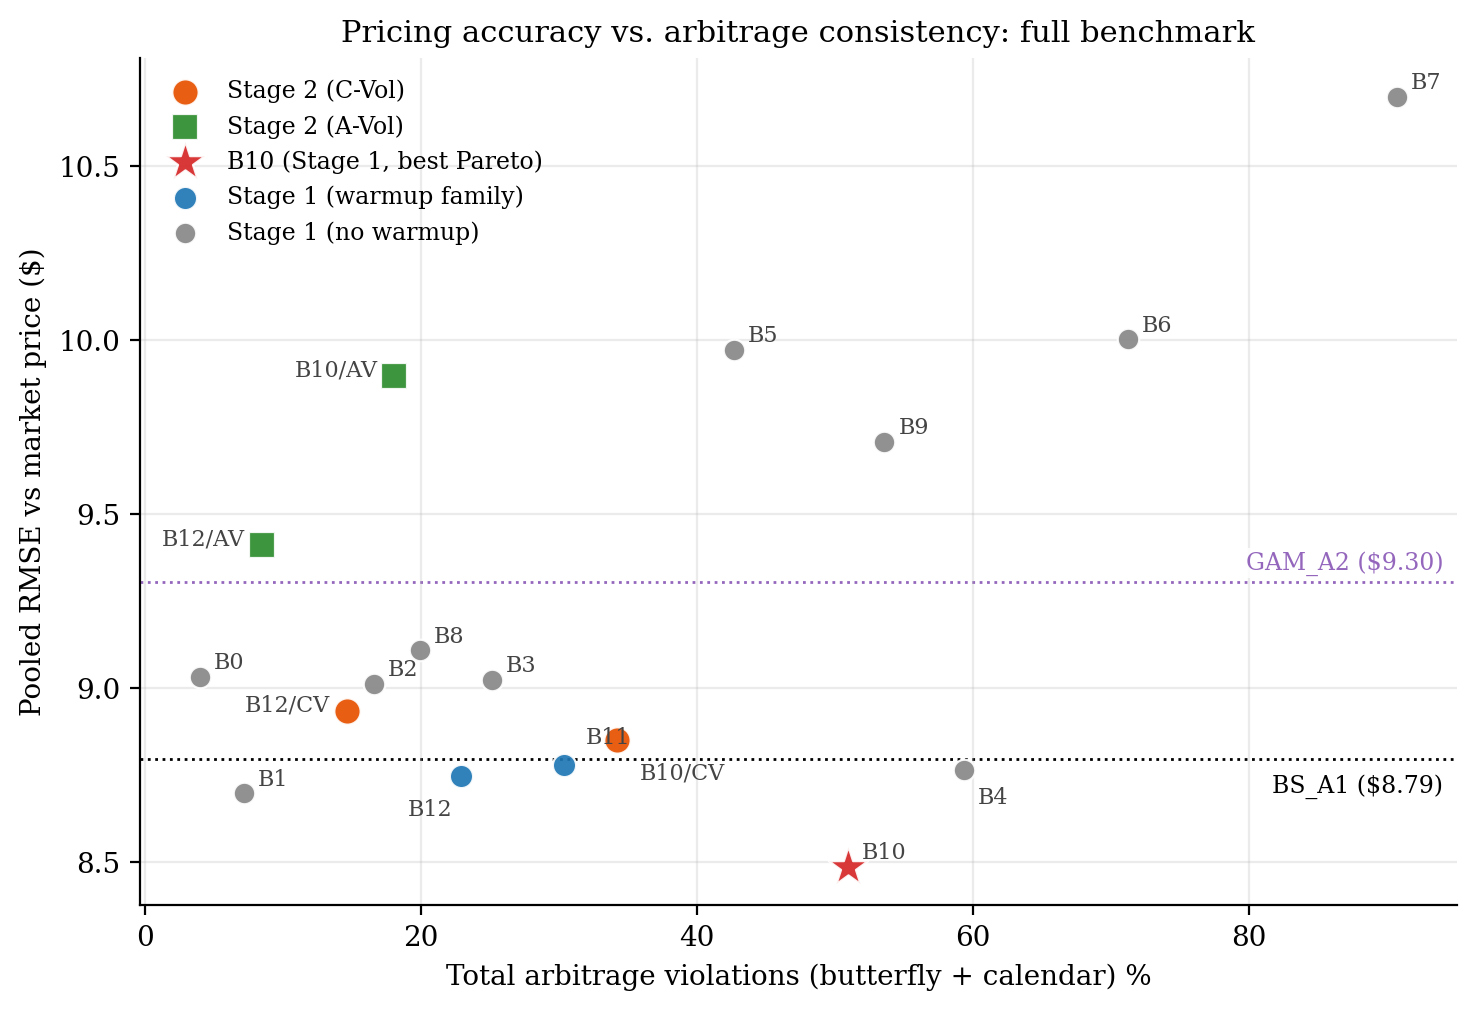
\includegraphics[width=0.9\linewidth,height=\textheight,keepaspectratio]{figures/fig-arb-rmse-pareto.png}

}

\caption{\label{fig-arb-rmse-pareto}Pricing accuracy vs.~arbitrage
consistency across the full benchmark. B10 (red star) is the lowest-RMSE
Stage 1 configuration; the warmup family (B11, B12, blue) trades roughly
\$0.3 of RMSE for about 30 percentage points of arbitrage reduction.
Stage 2 C-Vol (orange circles) and A-Vol (green squares) extend the
frontier further left, with B12/A-Vol at 8.5\% total violations the
cleanest model in the benchmark. Hybrid configurations without
PDE-warmup (B5--B7) collapse to the upper-right ``worst'' quadrant.}

\end{figure}%

\subsection{The wing-inversion finding}\label{sec-wing-inversion}

Stage 1 fixes a single volatility \(\sigma_\mathrm{fixed}\) inside the
PDE for the entire fold. Under the hybrid loss every Stage 1 model is
therefore caught in a tug-of-war: the PDE residual
\(\mathcal{L}_\mathrm{pde}\) pulls the price surface back towards a
flat-volatility Black--Scholes solution that does not curve at the
wings, while \(\mathcal{L}_\mathrm{data}\) pulls it towards the
empirical, smile-shaped market surface. For most configurations the PDE
side wins and the model collapses to an essentially flat-\(\sigma\)
residual; market deviations are absorbed into a uniform error band that
is largest where the smile is steepest, producing the standard OTM
\(\geq\) ATM \(\geq\) ITM pattern in stratified RMSE.

Figure \ref{fig-stratified-rmse} decomposes pooled RMSE by moneyness
band. Across the GAM baseline and 16 of the 17 PINN cells (Stage 1
B0--B12 and Stage 2 B10/B12 × cvol/avol alike) RMSE follows the
classical pattern OTM \(\geq\) ATM \(\geq\) ITM: volatility-skew effects
dominate the residual error in the wings. B10 is the only configuration
where this ordering inverts: ATM RMSE (\$8.83) exceeds both OTM RMSE
(\$8.48) and ITM RMSE (\$8.21). Equivalently, the \emph{wing} RMSE,
pooled across OTM and ITM, drops below the ATM RMSE. This is the
structural signature of a PINN where the data-driven curvature has
\emph{overpowered} the constant-volatility constraint precisely in the
wings, where the smile has the most curvature. The cost is paid in
arbitrage: B10's pricing network must fold smile-shaped local convexity
onto a single-\(\sigma\) PDE solution, and the resulting surface
registers the 33 percentage-point butterfly violation rate visible in
Figure \ref{fig-arb-rmse-pareto}. Configurations with the same \(\mu\)
but no warmup (B6), or warmup with different \(\mu\) (B11, B12), never
exhibit this inversion: in those cases the constraint side wins and the
wings are flattened. Neither do B10's Stage 2 successors, which we will
see absorb the same smile information into the volatility surface itself
(Section \ref{sec-stage2}) and therefore revert to the classical pattern
without paying the arb cost.

\begin{figure}[H]

\centering{

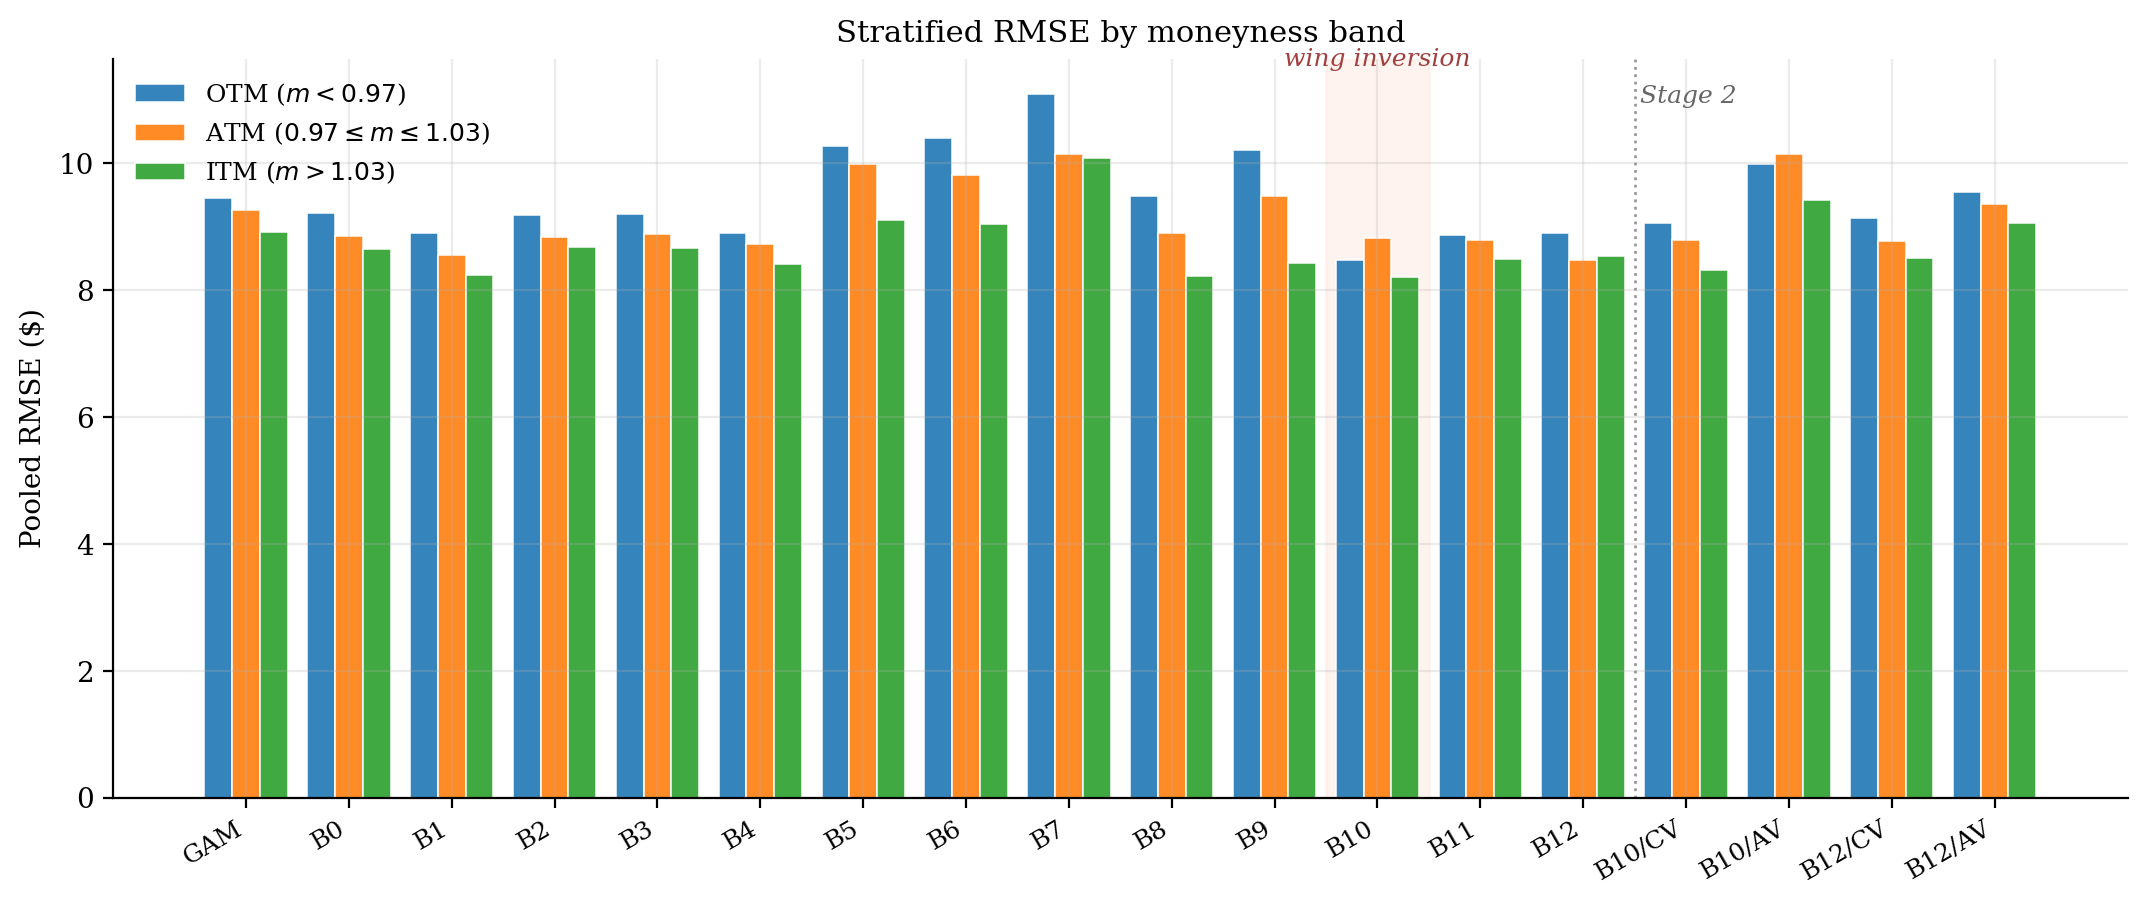
\includegraphics[width=1\linewidth,height=\textheight,keepaspectratio]{figures/fig-stratified-rmse.png}

}

\caption{\label{fig-stratified-rmse}Stratified RMSE across moneyness
bands. The standard pattern (RMSE OTM \(\geq\) ATM \(\geq\) ITM) holds
for every configuration except B10 (highlighted band), where the wings
beat the centre, the structural signature of recovered volatility-smile
curvature.}

\end{figure}%

\subsection{Stability and convergence diagnostics}\label{sec-stability}

The non-warmup hybrid configurations B5--B7 collapse on RMSE \emph{and}
on arbitrage simultaneously (Figure \ref{fig-arb-rmse-pareto}). The
overfitting mechanism foreshadowed in Section \ref{sec-training}, in
which gradient-norm-balanced \(\lambda_\mathrm{data}\) drifts upward as
\(\mathcal{L}_\mathrm{data}\) falls more slowly than the PDE / TC / BC
residuals and suppresses the PDE-consistency signal, is directly visible
in the per-loss curves and adaptive-weight trajectories. Figure
\ref{fig-loss-curves-stability} contrasts B6 (failure mode: modified
hybrid, \(\mu=0.75\), no warmup) with B10 (same architecture plus the
5,000-epoch PDE-warmup defined in Section \ref{sec-training}) on the
November 2020 fold. In B6 the market-data loss enters at full strength
from epoch 1 and is poorly balanced by Equation \ref{eq-grad-norm}; the
adaptive weight \(\lambda_\mathrm{data}\) runs to \(\sim 10^{5}\)
(Figure \ref{fig-weight-traj-stability}), which numerically suppresses
the PDE residual. The dominance ratio \(\rho(t)\) collapses below unity
early in training and stays there (Figure \ref{fig-pde-dominance}); the
val curve reaches its minimum well before the loop terminates and
val-best snapshot selection (Section \ref{sec-training}, step 3)
restores a model trained from a regime where the no-arbitrage geometry
has already been corrupted; hence the 51\% combined arb-violation rate
at the reported epoch. The 5,000-epoch warmup window in B10 lets
\(\mathcal{L}_\mathrm{pde}\), \(\mathcal{L}_\mathrm{tc}\), and
\(\mathcal{L}_\mathrm{bc}\) converge to a stable balance \emph{before}
the data loss is admitted; once \(\mathcal{L}_\mathrm{data}\) enters,
\(\rho(t)\) stays above unity, \(\lambda_\mathrm{data}\) remains
bounded, and the val-best epoch falls at a point inside the
PDE-consistent basin established during warmup. Val-best snapshot
reporting and PDE-warmup are therefore complementary: the snapshot
mechanism guards against late-epoch overfitting in the
generic-supervised sense, and the warmup schedule prevents the
optimisation trajectory from leaving the no-arbitrage region in the
first place.

\begin{figure}[H]

\centering{

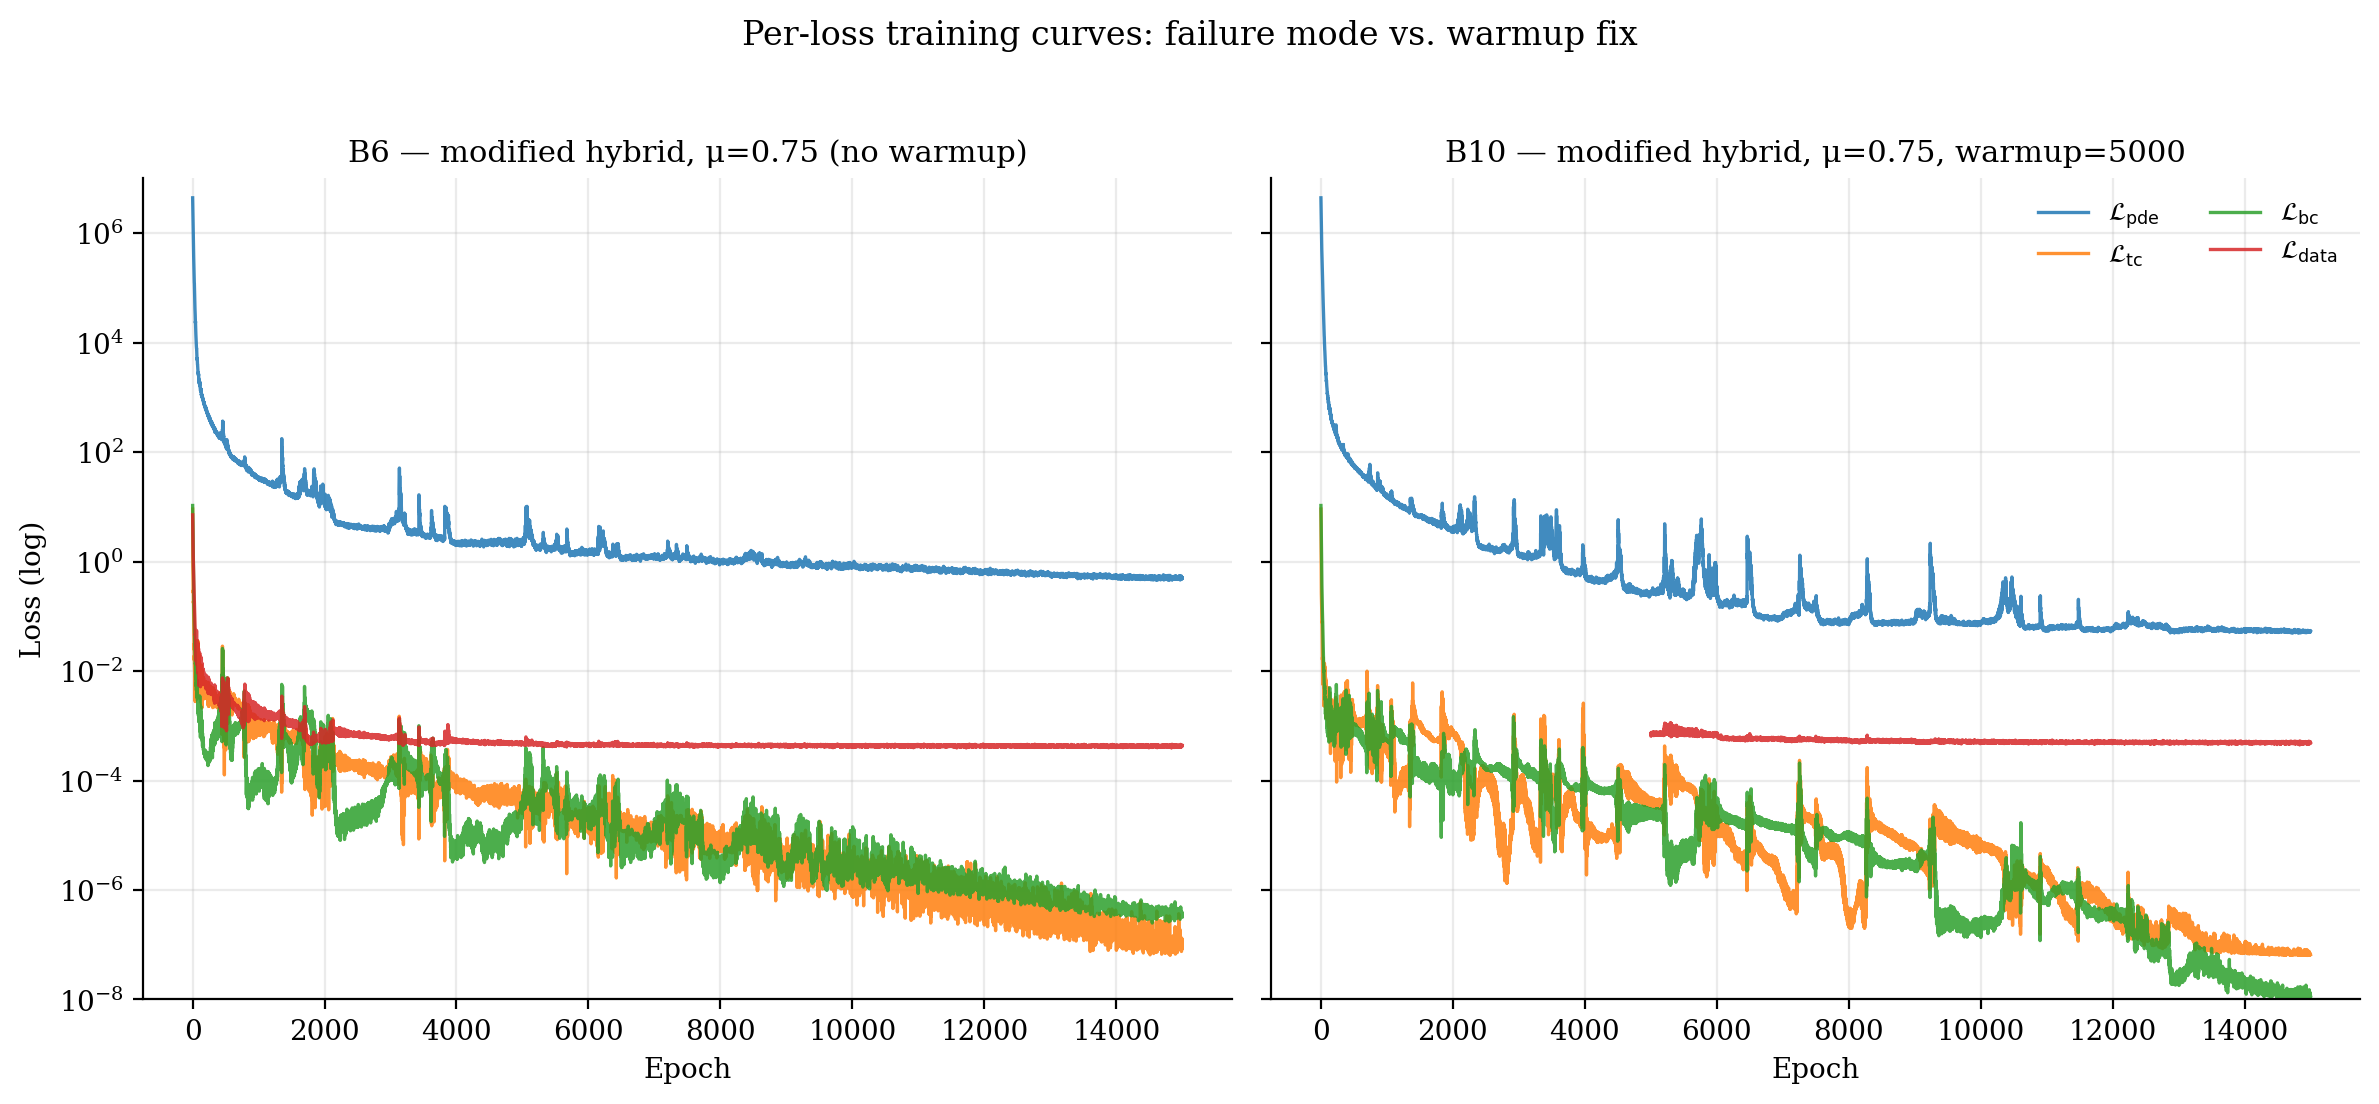
\includegraphics[width=0.8\linewidth,height=\textheight,keepaspectratio]{figures/fig-loss-curves-stability.png}

}

\caption{\label{fig-loss-curves-stability}Per-loss curves on Nov 2020.
Without warmup (B6, left), \(\mathcal{L}_\mathrm{data}\) dominates and
\(\mathcal{L}_\mathrm{pde}\) is starved; warmup (B10, right) keeps all
losses on a comparable scale.}

\end{figure}%

\begin{figure}[H]

\centering{

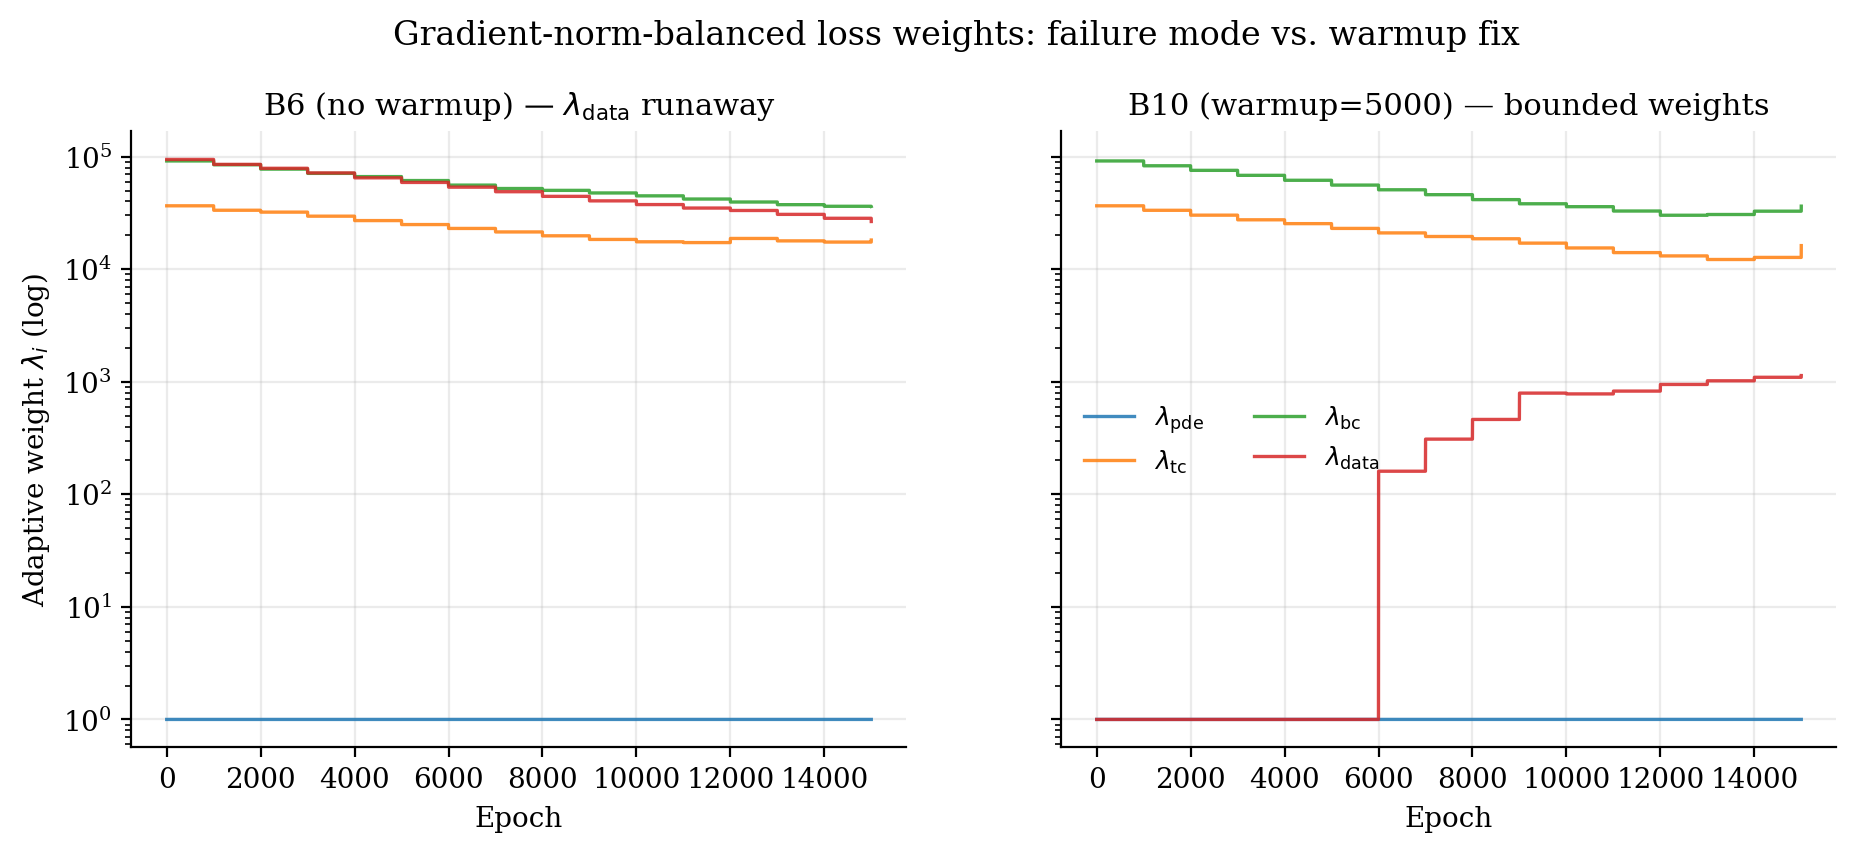
\includegraphics[width=0.8\linewidth,height=\textheight,keepaspectratio]{figures/fig-weight-traj-stability.png}

}

\caption{\label{fig-weight-traj-stability}Gradient-norm-balanced weights
\(\lambda_i\). Both runs initialise the TC and BC weights at large
values to compensate for their small raw gradients; in B6,
\(\lambda_\mathrm{data}\) stays at \(\sim 10^{5}\) (the \emph{runaway}
regime that suppresses PDE consistency), while in B10 the warmup phase
keeps \(\lambda_\mathrm{data}=0\) for 5,000 epochs and the post-warmup
data weight rises only to \(\sim 10^{3}\).}

\end{figure}%

\clearpage

\begin{figure}[H]

\centering{

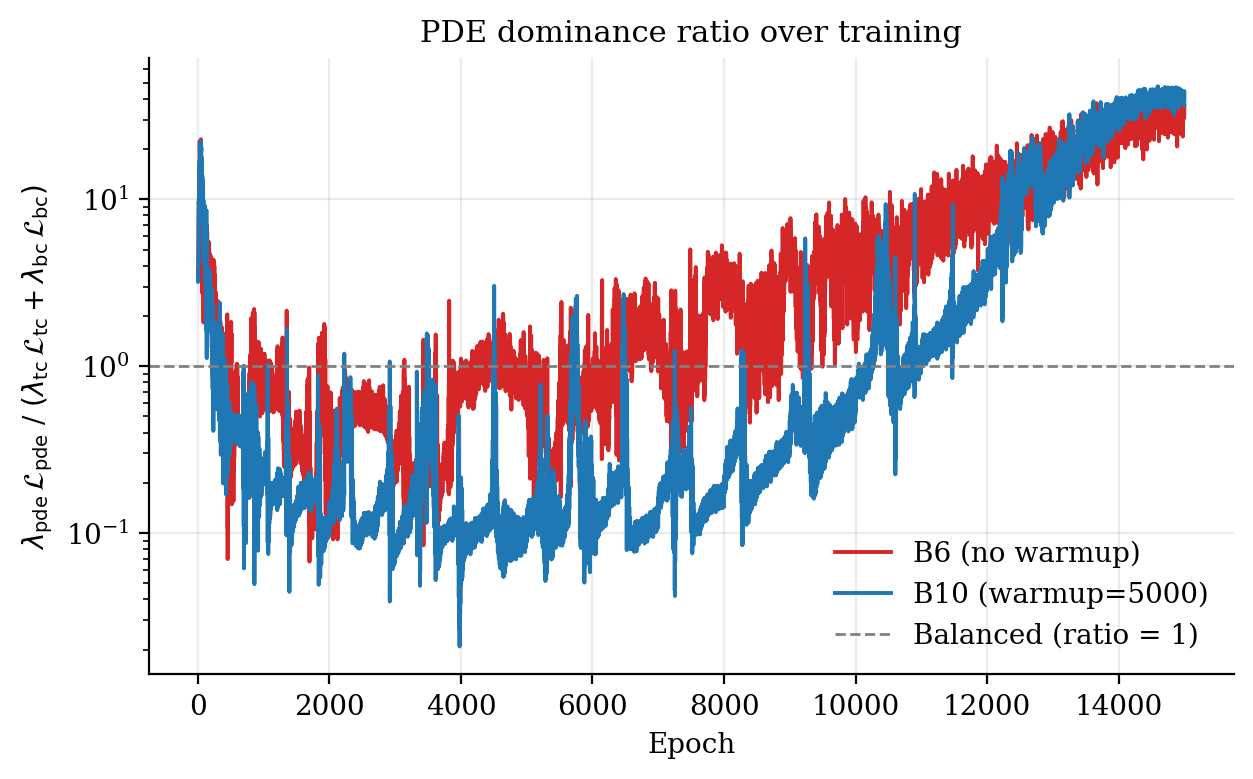
\includegraphics[width=0.8\linewidth,height=\textheight,keepaspectratio]{figures/fig-pde-dominance.png}

}

\caption{\label{fig-pde-dominance}PDE dominance ratio over training.
Both configurations transit through a low-ratio basin in early training
where the TC and BC residuals dominate the PDE residual; the warmup
window in B10 keeps the trajectory in this basin until epoch 5,000,
after which both runs climb together. The B6 trajectory is markedly
noisier; without the PDE-only basin to anchor it, the optimiser is
repeatedly pulled out of and back into PDE-consistent regions as
\(\lambda_\mathrm{data}\) shifts.}

\end{figure}%

\begin{figure}[H]

\centering{

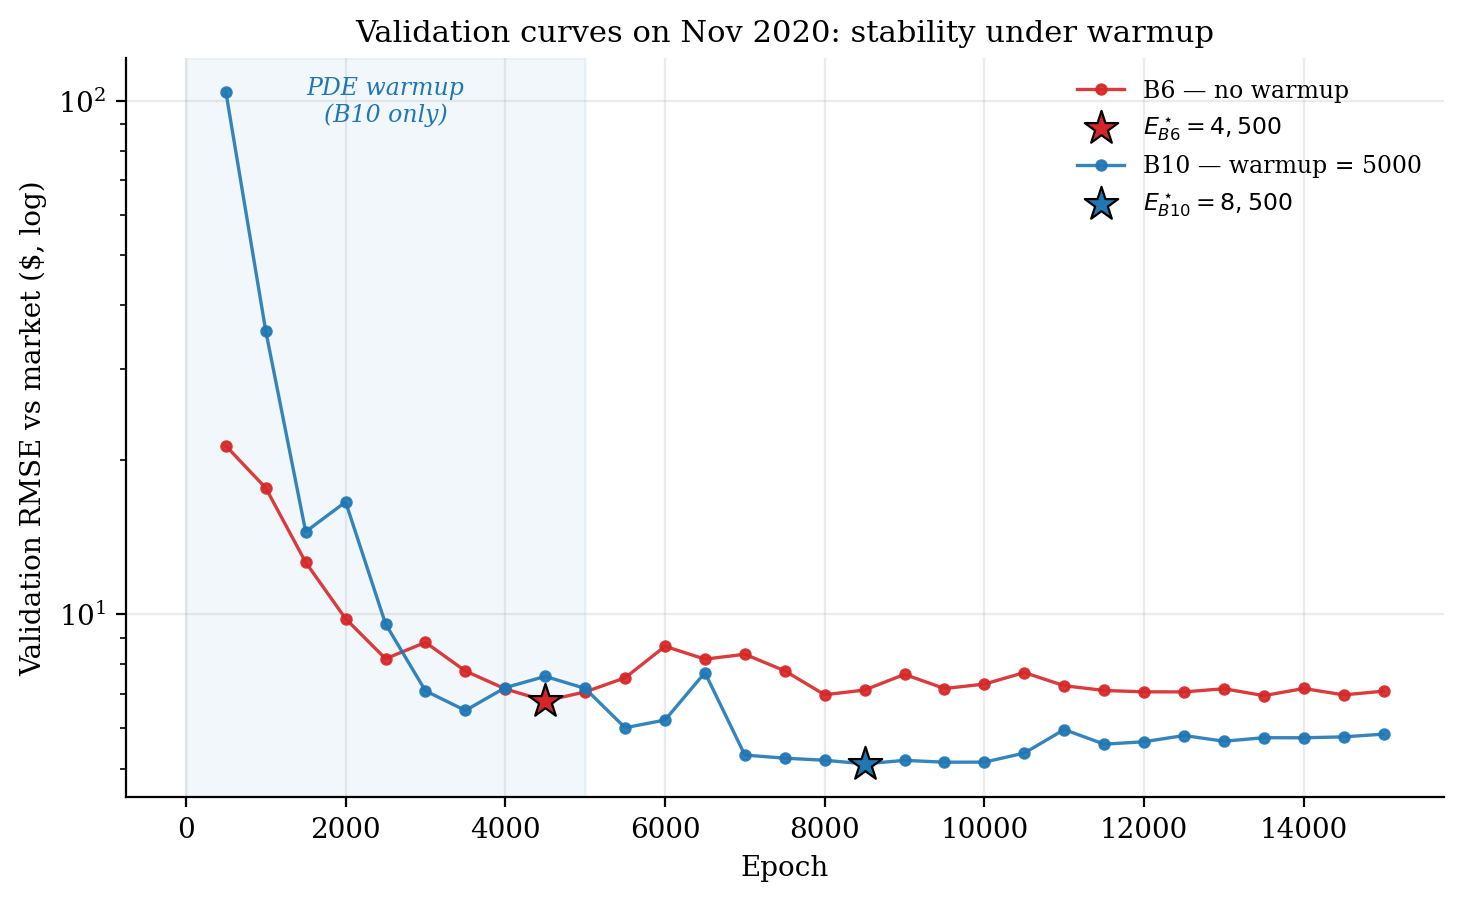
\includegraphics[width=0.8\linewidth,height=\textheight,keepaspectratio]{figures/fig-val-curve-mu-warmup.png}

}

\caption{\label{fig-val-curve-stability}Validation RMSE on Nov 2020 (log
scale) with the val-best epoch \(E^\star\) marked on each curve. B10's
val curve is monotonically smoother and reaches a lower minimum than
B6's, even though both start at the same RMSE; B6 plateaus higher and
noisier, the val-curve fingerprint of the unstable optimisation regime
documented in Figures
\ref{fig-loss-curves-stability}--\ref{fig-pde-dominance}. The shaded
band marks B10's PDE-warmup window.}

\end{figure}%

\subsection{\texorpdfstring{\(\mu \times \mathrm{warmup}\): substitutes,
not
complements}{\textbackslash mu \textbackslash times \textbackslash mathrm\{warmup\}: substitutes, not complements}}\label{sec-mu-warmup}

Within the warmup family (B10/B11/B12), pooled RMSE rises by \$0.26 as
\(\mu\) drops from 0.75 to 0.25, and the wing inversion is lost (Figure
\ref{fig-stratified-rmse}). The same direction is reflected in the
val-best epoch reported in Section \ref{sec-stage1} for each fold's
training: B10's mean \(E^\star\) across the nine folds is 6,167; B11's
is 6,222; B12's drops to 4,667. The lower-\(\mu\) initialisation is
closer to flat-\(\sigma\) BS, so the network has less to learn before
the val curve flattens. We conclude that \(\mu\)-tuning and the warmup
phase are substitutes: warmup does the heavy lifting of restoring
stability under hybrid losses, and \(\mu = 0.75\) is the companion that
maximises the pricing benefit; lowering \(\mu\) inside warmup gives back
most of the gain without an offsetting reduction in arbitrage.

\section{Stage 2: learnable volatility surface}\label{sec-stage2}

The Stage 1 ablation forced every PINN to express market-implied smile
structure inside a model that fixes a single \(\sigma_\mathrm{fixed}\).
The price the best-RMSE configuration paid to do this, visible as the
wing inversion of Section \ref{sec-wing-inversion} and the 51\% combined
arb-violation rate of Figure \ref{fig-arb-rmse-pareto}, is fundamentally
a representational mismatch: a smile-shaped surface cannot live in the
constant-volatility solution space without breaking the no-arbitrage
convexity of that space. Stage 2 acts as a pressure valve on this
mismatch. By replacing \(\sigma_\mathrm{fixed}\) inside the PDE with a
learnable surface \(\sigma_\theta(F,\tau)\), market complexity that
previously had to distort the price network is now absorbed directly
into the volatility specification, where it is properly bounded by the
SoftPlus parametrization. The pricing network can then return to a
genuinely PDE-consistent solution; the smile lives where it belongs, in
\(\sigma\).

We use the two endpoints of the Stage 1 frontier as Stage 2 warm-starts.
To keep their roles in mind, we attach functional labels:

\begin{itemize}
\tightlist
\item
  B10 (Max-Accuracy): modified-hybrid, \(\mu = 0.75\), warmup = 5,000.
  Lowest pooled RMSE in Stage 1 (\$8.49); pays for it with substantial
  arb violations (32\% butterfly, 19\% calendar) and the wing-inversion
  artefact.
\item
  B12 (Max-Consistency): modified-hybrid, \(\mu = 0.25\), warmup =
  5,000. RMSE only \$0.26 worse than B10 (\$8.75) but arb-clean (21\%
  butterfly, \emph{1.7\%} calendar) and free of wing inversion.
\end{itemize}

The \(2 \times 2\) design crosses these two warm-starts with the two
volatility parametrizations C-Vol and A-Vol, isolating the respective
contributions of the Stage 1 starting point and the inductive bias on
\(\sigma_\theta\).

\pagebreak

\begin{longtable}[]{@{}
  >{\raggedright\arraybackslash}p{(\linewidth - 12\tabcolsep) * \real{0.2771}}
  >{\raggedright\arraybackslash}p{(\linewidth - 12\tabcolsep) * \real{0.1807}}
  >{\raggedright\arraybackslash}p{(\linewidth - 12\tabcolsep) * \real{0.1205}}
  >{\raggedright\arraybackslash}p{(\linewidth - 12\tabcolsep) * \real{0.1084}}
  >{\raggedright\arraybackslash}p{(\linewidth - 12\tabcolsep) * \real{0.1084}}
  >{\raggedright\arraybackslash}p{(\linewidth - 12\tabcolsep) * \real{0.1084}}
  >{\raggedright\arraybackslash}p{(\linewidth - 12\tabcolsep) * \real{0.0964}}@{}}
\caption{Stage 2 walk-forward results: \(2 \times 2\) design crossing
the two Stage 1 warm-starts (B10 = Max-Accuracy, B12 = Max-Consistency)
with the two volatility parametrizations (C-Vol,
A-Vol).}\label{tbl-stage2}\tabularnewline
\toprule\noalign{}
\begin{minipage}[b]{\linewidth}\raggedright
Config
\end{minipage} & \begin{minipage}[b]{\linewidth}\raggedright
pooled RMSE
\end{minipage} & \begin{minipage}[b]{\linewidth}\raggedright
ATM
\end{minipage} & \begin{minipage}[b]{\linewidth}\raggedright
OTM
\end{minipage} & \begin{minipage}[b]{\linewidth}\raggedright
ITM
\end{minipage} & \begin{minipage}[b]{\linewidth}\raggedright
butt\%
\end{minipage} & \begin{minipage}[b]{\linewidth}\raggedright
cal\%
\end{minipage} \\
\midrule\noalign{}
\endfirsthead
\toprule\noalign{}
\begin{minipage}[b]{\linewidth}\raggedright
Config
\end{minipage} & \begin{minipage}[b]{\linewidth}\raggedright
pooled RMSE
\end{minipage} & \begin{minipage}[b]{\linewidth}\raggedright
ATM
\end{minipage} & \begin{minipage}[b]{\linewidth}\raggedright
OTM
\end{minipage} & \begin{minipage}[b]{\linewidth}\raggedright
ITM
\end{minipage} & \begin{minipage}[b]{\linewidth}\raggedright
butt\%
\end{minipage} & \begin{minipage}[b]{\linewidth}\raggedright
cal\%
\end{minipage} \\
\midrule\noalign{}
\endhead
\bottomrule\noalign{}
\endlastfoot
B10 (Max-Acc.)/C-Vol & \$8.851 & \$8.793 & \$9.065 & \$8.317 & 20.9\% &
13.4\% \\
B10 (Max-Acc.)/A-Vol & \$9.898 & \$10.155 & \$9.986 & \$9.425 & 13.2\% &
4.8\% \\
B12 (Max-Cons.)/C-Vol & \$8.935 & \$8.776 & \$9.146 & \$8.504 & 13.6\% &
1.0\% \\
B12 (Max-Cons.)/A-Vol & \$9.411 & \$9.367 & \$9.553 & \$9.069 & 8.2\% &
0.3\% \\
\end{longtable}

C-Vol vs A-Vol: the inductive-bias finding. Across both warm-starts the
multiplicative C-Vol parametrization delivers consistently lower RMSE
than the additive A-Vol parametrization at the cost of higher residual
arbitrage: B10 (Max-Accuracy) / C-Vol \$8.85 vs.~B10 / A-Vol \$9.90 on
pooled RMSE (C-Vol −\$1.05); B12 (Max-Consistency) / C-Vol \$8.94 vs.
B12 / A-Vol \$9.41 (−\$0.47). The arb--RMSE ordering reverses on the
consistency axis: A-Vol attains the lowest arbitrage-violation rates of
any model in the benchmark (B12 / A-Vol: 8.2\% butterfly + 0.3\%
calendar = 8.5\% total), while C-Vol stays in the 14--34\% range. The
interpretation is structural: the multiplicative form
\(\sigma_0\,\mathrm{softplus}(g_\theta)\) with \(\sigma_0\) anchored at
the per-fold ATM-IV median sits in a smaller, smoother subset of the
allowable \(\sigma\)-surface space: easier to optimise to low RMSE,
harder to bend into arbitrage-violating geometries.

Warm-start dependence. Stage 2 inherits the Pareto-frontier ordering
from Stage 1: the B10 (Max-Accuracy) warm-start produces lower-RMSE /
higher-arb Stage 2 models, and the B12 (Max-Consistency) warm-start
yields cleaner Stage 2 models. The two warm-starts \emph{reach} their
respective Stage 2 endpoints by qualitatively different mechanisms:
under B10 / C-Vol the volatility network learns a substantial multiplier
surface with \(\mu_{C}(F,\tau) \in [0.5, 1.0]\) (Figure
\ref{fig-vol-surface-b10-cvol}), i.e.~a learned \(\sigma\) ranging from
\(0.39\) to \(0.78\), effectively redistributing the smile structure
that the Max-Accuracy pricing net had previously encoded as
arb-violating curvature. Under B12 (Max-Consistency) / C-Vol the
multiplier collapses to \(\approx 1.000\pm 0.005\): the B12 warm-start
was already close to flat-\(\sigma\) BS, so the volatility network has
nothing to add and remains essentially inert. The Stage 1 endpoints
therefore behave as two distinct warm-start regimes for Stage 2, and the
\(2\times 2\) design separates the respective contributions of warm
start and parametrization.

\begin{figure}[H]

\centering{

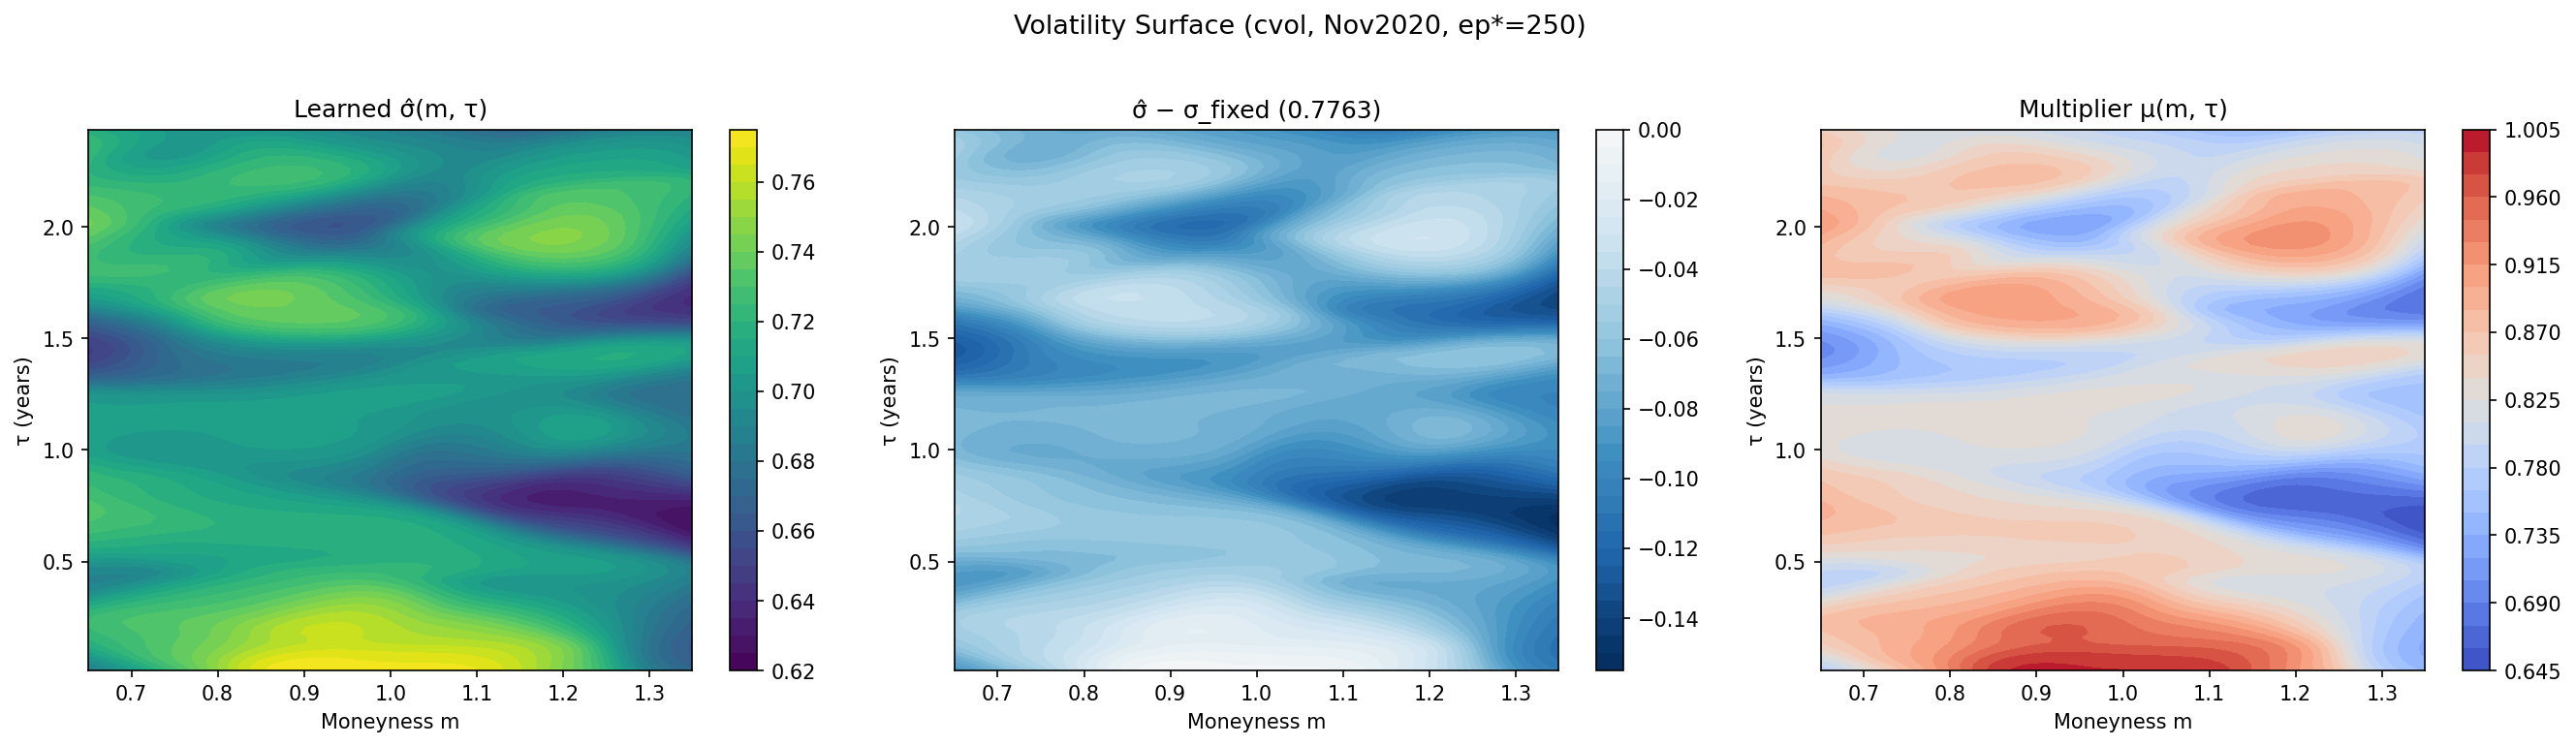
\includegraphics[width=0.95\linewidth,height=\textheight,keepaspectratio]{figures/fig-vol-surface-b10-cvol.png}

}

\caption{\label{fig-vol-surface-b10-cvol}Learned multiplicative
volatility surface \(\mu_C(F,\tau)\) for the B10 / C-Vol Stage 2 model
on the November 2020 fold. The vol network has absorbed substantial
smile and term structure, with the multiplier ranging 0.5--1.0 on top of
the per-fold \(\sigma_0=0.776\) anchor (right panel), producing realised
volatilities of roughly 0.39--0.78 across the moneyness × maturity grid
(left panel).}

\end{figure}%

\begin{figure}[H]

\centering{

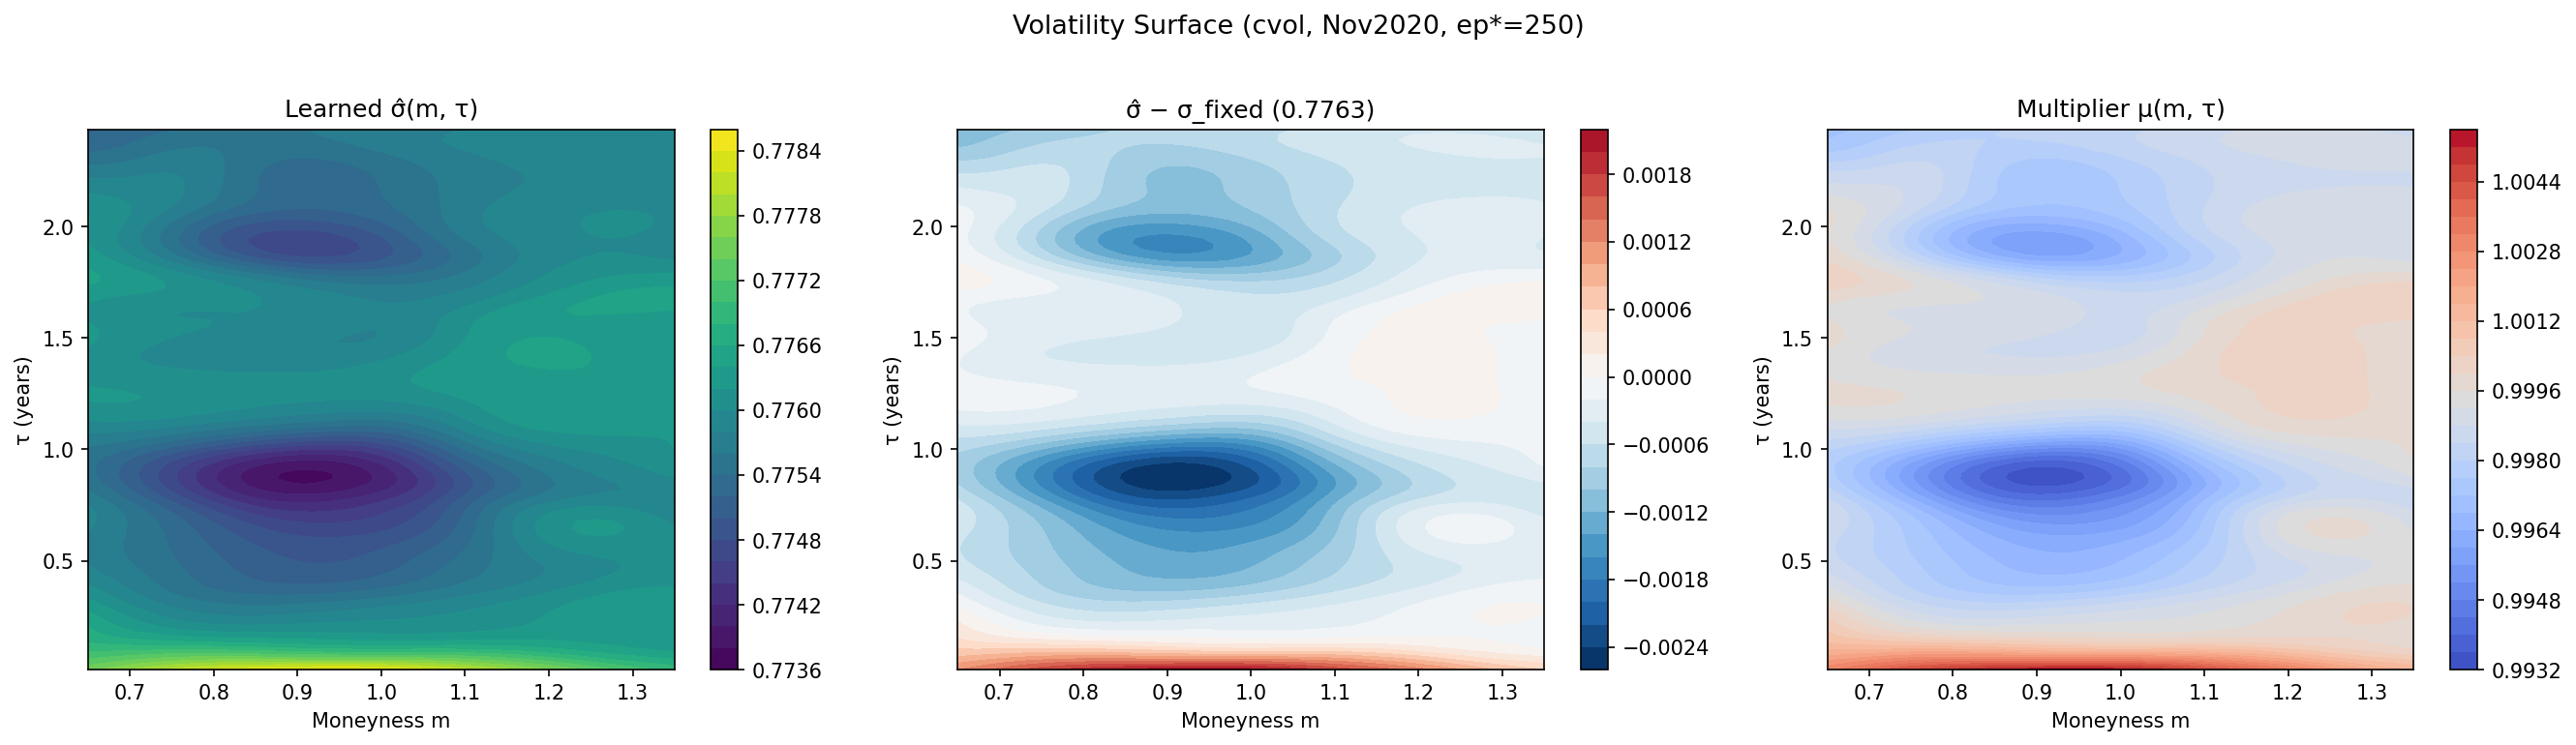
\includegraphics[width=0.95\linewidth,height=\textheight,keepaspectratio]{figures/fig-vol-surface-b12-cvol.png}

}

\caption{\label{fig-vol-surface-b12-cvol}Stage 2 / C-Vol multiplier on
the same fold under the cleaner B12 warm-start. The vol network stays
essentially inert (\(\mu_C \approx 1.000\pm 0.005\), right panel),
reflecting that the B12 pricing net already sits close to
flat-\(\sigma\) Black--Scholes, so the volatility network has little
structural correction to add.}

\end{figure}%

Wing-inversion under Stage 2. The Stage 1 wing inversion identified for
B10 (Max-Accuracy) in Section \ref{sec-wing-inversion} does \emph{not}
survive Stage 2: B10 / C-Vol returns to the classical OTM \(\geq\) ATM
\(\geq\) ITM pattern (\$9.07 / \$8.79 / \$8.32). This is the
pressure-valve effect made concrete: the structural deviation from
flat-\(\sigma\) that manifested as a wing-inversion artefact in the
Max-Accuracy Stage 1 pricing net is absorbed by the volatility network
in B10 / C-Vol, where it is properly bounded by the no-arbitrage
constraints implicit in the SoftPlus parametrization. The smile moves
from the price surface (where it caused arb violations) to the
volatility surface (where it is admissible).

Convergence speed. All four Stage 2 configurations select their val-best
epoch substantially earlier than the corresponding Stage 1
configurations: \(E^\star \in \{2,222, 2,389, 2,444, 4,861\}\) for the
four Stage 2 cells vs.~\(\{4,667, 6,167\}\) for the B12 / B10 Stage 1
warm-starts. The warm-started pricing net gives the joint optimisation a
near-optimal initialisation, and the volatility network, operating in a
much lower-dimensional output space than the pricing net, converges
quickly within that basin.

\section{Non-PINN baselines}\label{sec-baselines}

\begin{longtable}[]{@{}llll@{}}
\caption{Non-PINN baselines under identical walk-forward folds and
strict feature set.}\label{tbl-baselines}\tabularnewline
\toprule\noalign{}
Config & RMSE & ATM & Wing \\
\midrule\noalign{}
\endfirsthead
\toprule\noalign{}
Config & RMSE & ATM & Wing \\
\midrule\noalign{}
\endhead
\bottomrule\noalign{}
\endlastfoot
BS & 8.795 & --- & --- \\
GAM & 9.305 & 9.272 & 9.313 \\
LAGP & 11.305 & 11.113 & 11.350 \\
\end{longtable}

The Black--Scholes (BS) baseline is more competitive than its reputation
suggests: at \$8.79 pooled RMSE it sits \emph{below} every Stage 1 PINN
configuration except B10 (Max-Accuracy), and at most \$0.16 above any
Stage 2 cell. Two design choices drive this. The calibration uses the
\emph{median ATM implied volatility on the training data} as
\(\sigma_\mathrm{fixed}\), the right one-parameter summary of the smile
if a single number must be chosen, and the fixed risk-free rate
\(r_\mathrm{fixed}\) is taken from the same training window. Both are
recomputed per fold, so Black--Scholes adapts to regime even though the
model itself does not. This makes it a substantially harder benchmark
than the typical ``closed-form with a textbook 0.20 vol'' comparator
reported in much of the PINN-pricing literature, and is part of why our
Stage 1 RMSE comparison reads tighter than expected.

The Residual GAM under-performs at \$9.31, half a dollar worse than
Black--Scholes, under the \emph{strict} feature set we impose
(\(m,\ \tau,\ \log v\)). This is the same GAM specification that, in
earlier formulations, beat BS by a wide margin once a discrete regime
indicator was added to the design matrix. Removing that indicator
removes most of the gap: the smooth smile-and-term structure that the
GAM can fit on its own does not buy back what flat-\(\sigma\)
Black--Scholes was already capturing, and the absence of regime
information costs it on the high-volatility folds. We retain the strict
GAM rather than the regime-augmented one because the PINN information
set does not include a regime indicator either; using it for the GAM
would compare two models with different inputs rather than two models on
the same problem.

The Residual laGP gives the worst point-estimate RMSE in the entire
benchmark (\$11.31) but is nevertheless retained because it is the
\emph{only} baseline that produces a native 95\% predictive interval at
every test option. Its 95\% empirical coverage is well-calibrated under
the strict feature set, and its mean PI width is the natural reference
yardstick for the anchored-ensemble extension we discuss in Section
\ref{sec-uq-future}. We treat Residual laGP as the credible-interval
benchmark, not the point-estimate benchmark.

\pagebreak

\section{Discussion}\label{sec-discussion}

\subsection{Pooled versus mean-fold
RMSE}\label{pooled-versus-mean-fold-rmse}

The pooled RMSE we report throughout, \(\sqrt{\sum_f \sum_i e_{f,i}^2 /
\sum_f n_f}\), weights each fold by its test-month sample size, which is
the correct estimator if one views the nine months as a single test
pool. The \emph{mean fold} RMSE \((1/9)\sum_f \mathrm{RMSE}_f\) is
sometimes more informative because it equally weights heterogeneous
regimes: in our data the standard deviation across folds is large
(e.g.~\$3.94 for B10 Max-Accuracy on a pooled value of \$8.49), and a
single fold (September 2020, the COVID-rebound peak) drives most of that
spread. Sep 2020 produces RMSEs around \$14--18 across every
configuration we trained, including non-PINN baselines, and is clearly
the limit-of-difficulty fold of our 2020 dataset.

Mean-fold RMSE compresses this heterogeneity: B10 Max-Accuracy's
mean-fold RMSE is \$6.75 (vs.~\$8.49 pooled), and every Stage 2 cell
sits in the \$6.85--\$7.76 mean-fold range. The mean-fold ranking is
qualitatively the same as the pooled ranking, with B10 and B12
(Max-Consistency) at the top of Stage 1 and B10 / C-Vol best of Stage 2;
the absolute gaps shrink, however, because the Max-Accuracy
pricing-and-arb tradeoff is most pronounced exactly on the hardest
folds. We report pooled RMSE as the primary metric; it is consistent
with how a practitioner who pooled all nine months of out-of-sample
residuals together would summarise the model. Mean-fold RMSE is reported
alongside as a robustness check.

\subsection{Limitations}\label{limitations}

Limitations bound the conclusions of this study. To begin with, the
dataset is a single underlying (TSLA, an unusually volatile
S\&P-inclusion-year stock), so generalisation to indices, low-vol single
names, or multi-name baskets is not addressed. In addition, the
walk-forward window covers a regime-rich but historically unique period
(the COVID crash followed by the autumn S\&P-inclusion melt-up);
fold-size heterogeneity is therefore severe, with Apr 2020 carrying only
12,743 training observations against Dec 2020's 50,000+. The conclusions
about Stage 2's value are most robust on the data-rich late-2020 folds,
and weaker on the small-data early folds; we have argued in Section
\ref{sec-stage2} that the size of the Stage-2 RMSE penalty on small
folds is consistent with capacity-versus-data scaling rather than a
genuine deficiency of the architecture, but a calmer regime would test
this more cleanly. Moreover, the benchmark is purely statistical: we
evaluate point and interval quality against quoted mid-prices and never
simulate hedging errors, transaction costs, or strategy P\&L. A
hedging-quality evaluation would convert RMSE into something with
directly interpretable economic units, and would weight the arbitrage
metrics differently because surface-consistency violations manifest as
concrete hedging losses rather than coverage failures. Most importantly,
while the 5,000-epoch PDE-warmup successfully stabilized the
Pareto-optimal configurations, the underlying gradient-norm balancing
mechanism is fundamentally unstable for hybrid option pricing. As seen
in the complete collapse of configurations B5 through B8, attempting to
balance \(\mathcal{L}_{data}\) and \(\mathcal{L}_{pde}\) simultaneously
from initialization universally triggers a runaway data-weight effect.
The warmup schedule acts as a functional heuristic to bypass this, but
it highlights that current dynamic loss-balancing algorithms are
structurally insufficient for this problem space without rigid
phase-scheduling.

\subsection{Future direction: uncertainty
quantification}\label{sec-uq-future}

The walk-forward and val-best protocol above produces a single point
estimate per fold. A natural extension applies anchored ensembles
(Kazemian and Author Et Al. 2024): train \(K\) replicas of the Stage 2
PINN, each with a Gaussian anchor on its initial weights, and read 95\%
predictive intervals from the empirical quantiles across the ensemble.
The existing laGP baseline (Section \ref{sec-baselines-method}) provides
a non-PINN credible-interval comparator under the \emph{same} fold
definitions and information set, so the comparison is calibrated on
coverage rate and average interval width without re-running the non-PINN
side. This is the planned next step; we leave its implementation,
ensemble-size sweep, and coverage-vs-width analysis to subsequent work.
Alongside uncertainty quantification, future methodological work will
explore more robust loss-balancing mechanisms for hybrid PINNs.

\section{Conclusion}\label{sec-conclusion}

We benchmarked physics-informed neural networks for European option
pricing on a single-name equity dataset (TSLA, 2020) under a strict
walk-forward protocol with single-phase val-best snapshot reporting, and
compared against per-fold-\(\sigma\) Black--Scholes, a residual GAM
under the strict feature set, and a residual local approximate GP. Three
findings stand out.

The PINN pricing problem is governed by a sharp tradeoff between market
accuracy and arbitrage consistency, and the gradient-norm loss-balancing
scheme is the lever that controls where on that tradeoff a configuration
lands. Without intervention the scheme amplifies
\(\lambda_\mathrm{data}\) to \(\sim 10^{5}\) within the first few
thousand epochs, the PDE-dominance ratio collapses below unity, and the
resulting model has both high RMSE \emph{and} high arb violations: the
upper-right ``worst'' quadrant of Figure \ref{fig-arb-rmse-pareto},
where every non-warmup hybrid configuration (B5--B7) ends up. A
5,000-epoch PDE-warmup schedule that keeps the data loss deactivated
until the PDE/TC/BC weights have settled is structurally sufficient to
prevent this collapse: the entire Pareto frontier of our benchmark (B10,
B11, B12 in Stage 1, and all four Stage 2 cells) consists of warmup
configurations. The combination of warmup + val-best snapshot reporting
also handles the two distinct overfitting modes (generic supervised
noise-fitting and PINN-specific gradient-norm runaway) without
conflating them.

Inside the warmup family, RWF \(\mu\) moves the model along the Pareto
frontier. B10 (Max-Accuracy, \(\mu = 0.75\)) achieves the lowest pooled
RMSE in the entire benchmark (\$8.49) but pays for it with a 51\%
combined arbitrage-violation rate and a wing-inversion artefact in
stratified RMSE, the structural fingerprint of a PINN whose pricing
network has bent the constant-\(\sigma\) PDE solution to fit empirical
smile curvature. B12 (Max-Consistency, \(\mu = 0.25\)) gives back \$0.26
of pooled RMSE in exchange for an essentially clean calendar surface
(1.7\% calendar arb) and no wing inversion. \(\mu\)-tuning and the
warmup phase are \emph{substitutes}, not complements: lowering \(\mu\)
inside the warmup regime does not stack a second improvement on top of
the first.

Stage 2 absorbs market complexity directly into a learnable volatility
surface \(\sigma_\theta(F,\tau)\), and the parametrization of that
surface controls the inductive bias. The multiplicative C-Vol wrapper
\(\sigma_0\,\mathrm{softplus}(g_\theta)\), anchored at the per-fold
ATM-IV median, gives lower RMSE than the additive A-Vol form across both
warm-starts; A-Vol gives lower arbitrage-violation rates, with B12
(Max-Consistency) / A-Vol the cleanest model in the entire benchmark
(8.5\% combined violations). The B10 / C-Vol configuration in particular
shows that the smile structure that the Max-Accuracy Stage 1 pricing
network had encoded as arb-violating curvature is redistributed into the
volatility surface as a multiplier ranging \$\sim\$0.5--1.0, and the
wing inversion disappears: empirical confirmation that the Stage-1
artefact and the Stage-2 mechanism are two views of the same
representational problem. Stage 2 also converges substantially faster
than Stage 1 (val-best epoch roughly halved), reflecting that the
warm-started pricing network places joint optimisation near a
well-conditioned basin in which the volatility network needs only small
structural corrections.

The natural extension is uncertainty quantification: anchored ensembles
applied to the Stage 2 architecture, with coverage and interval width
benchmarked against the laGP credible intervals already computed under
the same walk-forward protocol. The methodology developed here (strict
walk-forward folds, val-best reporting, gradient-norm + warmup loss
balancing, and arbitrage violations as a primary metric on equal footing
with RMSE) applies unchanged to that extension and to subsequent
multi-name or hedging-quality evaluations.

\pagebreak

\section*{Acknowledgments}\label{acknowledgments}
\addcontentsline{toc}{section}{Acknowledgments}

The author acknowledges the use of Claude Code (Anthropic) as an AI
assistant for code generation, debugging, and implementation support
during the software development phase of this research. All generated
code was thoroughly reviewed, tested, and validated by the author.

\section*{References}\label{references}
\addcontentsline{toc}{section}{References}

\phantomsection\label{refs}
\begin{CSLReferences}{1}{0}
\bibitem[\citeproctext]{ref-blackscholes1973}
Black, Fischer, and Myron Scholes. 1973. {``The Pricing of Options and
Corporate Liabilities.''} \emph{Journal of Political Economy} 81 (3):
637--54.

\bibitem[\citeproctext]{ref-dupire1994}
Dupire, Bruno. 1994. {``Pricing with a Smile.''} \emph{Risk Magazine} 7
(1): 18--20.

\bibitem[\citeproctext]{ref-gramacy2016lagp}
Gramacy, Robert B. 2016. {``{laGP}: Large-Scale Spatial Modeling via
Local Approximate {G}aussian Processes in {R}.''} \emph{Journal of
Statistical Software} 72 (1): 1--46.

\bibitem[\citeproctext]{ref-heston1993}
Heston, Steven L. 1993. {``A Closed-Form Solution for Options with
Stochastic Volatility with Applications to Bond and Currency Options.''}
\emph{Review of Financial Studies} 6 (2): 327--43.

\bibitem[\citeproctext]{ref-kazemian2024}
Kazemian, Pegah, and Author Et Al. 2024. {``Uncertainty-Aware
Physics-Informed Neural Networks for Option Pricing.''} \emph{Working
Paper}.

\bibitem[\citeproctext]{ref-merton1973}
Merton, Robert C. 1973. {``Theory of Rational Option Pricing.''}
\emph{Bell Journal of Economics and Management Science} 4 (1): 141--83.

\bibitem[\citeproctext]{ref-raissi2019}
Raissi, Maziar, Paris Perdikaris, and George E. Karniadakis. 2019.
{``Physics-Informed Neural Networks: A Deep Learning Framework for
Solving Forward and Inverse Problems Involving Nonlinear Partial
Differential Equations.''} \emph{Journal of Computational Physics} 378:
686--707. \url{https://doi.org/10.1016/j.jcp.2018.10.045}.

\bibitem[\citeproctext]{ref-tancik2020fourier}
Tancik, Matthew, Pratul Srinivasan, Ben Mildenhall, Sara Fridovich-Keil,
Nithin Raghavan, Utkarsh Singhal, Ravi Ramamoorthi, Jonathan Barron, and
Ren Ng. 2020. {``Fourier Features Let Networks Learn High Frequency
Functions in Low Dimensional Domains.''} \emph{NeurIPS}.

\bibitem[\citeproctext]{ref-wang2023expert}
Wang, Sifan, Shyam Sankaran, Hanwen Wang, and Paris Perdikaris. 2023.
{``An Expert's Guide to Training Physics-Informed Neural Networks.''}
\emph{arXiv Preprint arXiv:2308.08468}.

\bibitem[\citeproctext]{ref-wood2017gam}
Wood, Simon N. 2017. \emph{Generalized Additive Models: An Introduction
with r}. 2nd ed. Chapman; Hall/CRC.

\end{CSLReferences}




\end{document}
